\chapter{Precoding for MU-MIMO systems}
\label{chapter:mu_mimo_precoding}

Consider the downlink \ac{MU}-\ac{MIMO} system introduced in Section~\ref{subsection:mu_mimo_system_model}.
The key difference from the \ac{SU}-\ac{MIMO} system of the previous chapter is the presence of inter-user interference: the signal intended for one user leaks into the receive antennas of the other users.

The preceding chapter restricted attention to linear precoding, in which the transmitted signal is obtained by applying a linear transformation, represented by a matrix, to the data symbol vector.
Nonlinear precoding techniques, on the other hand, apply nonlinear processing to the data symbols before transmission.
While linear precoding can achieve the capacity of the \ac{SU}-\ac{MIMO} channel, it is no longer capacity-achieving in the \ac{MU}-\ac{MIMO} setting.

Two well-known nonlinear precoding techniques are \acf{DPC}~\cite{dirty_paper_costa} and \acf{THP}~\cite{THP_harashima, THP_MIMO}.
\ac{DPC} is an information-theoretic technique that achieves the capacity region of the Gaussian broadcast channel by encoding each data stream such that interference from all previously encoded streams is pre-subtracted at the transmitter.
\ac{THP} approximates \ac{DPC} at reduced complexity by successively canceling inter-user interference at the transmitter using modulo arithmetic.
Despite their superior capacity, nonlinear techniques incur a significantly higher computational cost.
Linear precoding, by contrast, offers near-optimal performance at a fraction of the complexity, and therefore remains the preferred approach in practice.
This chapter accordingly focuses on linear precoding techniques.

The following sections present four commonly used linear precoding strategies for the \ac{MU}-\ac{MIMO} downlink, arranged in order of increasing complexity.
The presentation begins with three precoding techniques related to \acs{ZF}, and concludes with the state-of-the-art \acs{WMMSE} precoder.
At the end of this chapter, their performance is compared through numerical simulations for different system configurations.
In line with the previous chapter, the design is focused on maximizing the total \acf{SR} of the system.

\section{Zero-Forcing Precoding}
\label{subsection:mu_mimo_zf_precoding}
% =============================
%     Zero-Forcing
% =============================

The objective of \acf{ZF} precoding is to cancel all interference, both inter-user and inter-stream.
Moreover, no receiver-side combining is applied. Instead, all processing is done by the precoder and each \ac{UT} forwards its received samples directly for detection.

Considering these restrictions, we obtain that
\begin{equation}
\label{eq:zf_restrictions}
    \mathbf{T} = (\mathbf{G}\mathbf{H}\mathbf{F}) = \sqrt{\mathbf{Q}} \quad \text{and} \quad \mathbf{G} = \mathbf{I}_{\mathrm{rect}},
\end{equation}
where $\mathbf{T}$ is the compound \ac{MU}-\ac{MIMO} transfer matrix, $\sqrt{\mathbf{Q}} \in \mathbb{R}_{>0}^{K\,N_S \times K\,N_S}$ is a diagonal scaling matrix and $\mathbf{I}_{\mathrm{rect}}$ is a rectangular diagonal matrix with unit entries on its main diagonal.
The compound \ac{MU}-\ac{MIMO} input--output relation~\eqref{eq:mu_mimo_precoding_combining_io_compact} then simplifies to
\begin{equation}
\label{eq:zf_io}
    z_{k,\,i} = q_{k, i} \, a_{k, i} + n_{k, i} \qquad \text{for} \quad k = 1, \dots, K \quad \text{and} \quad i = 1, \dots, N_S.
\end{equation}
This shows that the interference has been completely eliminated and each data stream is received over an independent scalar \ac{AWGN} channel, which allows performing symbol-by-symbol detection at each \ac{UT}.

It is shown in~\cite{mu_mimo_ZF_precoding} that the constraints in~\eqref{eq:zf_restrictions} are satisfied when the precoder is chosen as the right pseudo-inverse of the channel matrix, scaled by $\sqrt{\mathbf{Q}}$:
\begin{equation}
\label{eq:zf_precoder}
    \mathbf{F} = \mathbf{H}^{\mathsf{H}} (\mathbf{H} \mathbf{H}^{\mathsf{H}})^{-1} \, \sqrt{\mathbf{Q}}
\end{equation}
This expression requires the channel matrix to have full row rank ($R_H = K\,N_S$), so that the inverse $(\mathbf{H}\mathbf{H}^{\mathsf{H}})^{-1}$ exists.
For an \ac{i.i.d.} Rayleigh fading channel, this condition holds almost surely provided that $N_T \geq K N_S$.
In what follows, this condition is assumed to be satisfied.
If it is not, the inverse $(\mathbf{H}\mathbf{H}^{\mathsf{H}})^{-1}$ is replaced by the Moore-Penrose pseudo-inverse, which is computed from the \ac{SVD} of the channel matrix~\cite{moore_penrose_pseudoinverse}.

It remains to determine the optimal diagonal entries of the scaling matrix $\mathbf{Q}$ so as to maximize the \acf{WSR} under the total transmit power constraint.
Considering~\eqref{eq:zf_io}, the \ac{WSR} of the system can be written as
\begin{equation}
\label{eq:zf_wsr}
    \mathrm{WSR} = \sum_{k=1}^{K} \sum_{i=1}^{N_S} \, \mu_{k, i} \, \log_2\big(1 + \frac{q_{k, i}}{N_0}\big),
\end{equation}
where $\mu_{k, i}$ is the weight assigned to the $i$th data stream intended for \ac{UT} $k$.
Substituting the \ac{ZF} precoder into the transmit power constraint~\eqref{eq:mu_mimo_power_constraint} yields %(see Appendix~\ref{appendix:calculations})
\begin{equation}
\label{eq:zf_power_constraint}
    \sum_{k=1}^{K} \sum_{i=1}^{N_S} \, q_{k, i} \, \big((\mathbf{H} \mathbf{H}^{\mathsf{H}})^{-1}\big)_{n,\,n} \leq P_t \qquad \text{with} \quad n = (k-1)\,N_S + i.
\end{equation}
Let us introduce the substitution
\begin{equation}
    p_n = \gamma_n^{-1} \, q_{k, i} \quad \text{with} \quad \gamma^{-1}_n = \big((\mathbf{H} \mathbf{H}^{\mathsf{H}})^{-1}\big)_{n,\,n},
\end{equation}
such that we can write the \ac{WSR} maximization problem as follows:
\begin{equation}
\begin{aligned}
    &\underset{\{p_n\}}{\max} \;\; \sum_{n=1}^{K\, N_S} \, \alpha_n \, \log_2\big(1 + \frac{\gamma_n}{N_0} \, p_n \big) \\
    &\mathrm{s. t.} \;\;\; \sum_{n=1}^{K\, N_S} \, p_n \leq P_t
\end{aligned}
\end{equation}
This is exactly the optimization problem handled in Appendix~\ref{appendix:waterfilling}.
The optimal values for $p_i$ are therefore obtained using the waterfilling solution as described in Algorithm~\ref{alg:waterfilling}.

Note that the above power allocation strategy may allocate almost no power to the data streams of a \ac{UT} with poor channel conditions.
The achievable rate for that specific user will therefore be very small, compared to the other users with better channel conditions.
An alternative, more fair approach is to divide the total transmit power equally across the different users, and use the waterfilling solution to allocate the power to which every user is entitled across the different data streams intended for that user.


To summarize, the steps required for computing the \ac{ZF} compound precoder matrix for total \ac{SR} maximization across all \acp{UT} are described in Algorithm~\ref{alg:zf_precoding}.
\begin{algorithm}[!htbp]
\caption{\ac{ZF} Precoding}
\label{alg:zf_precoding}
\begin{algorithmic}[1]
    
    \Require 
    \Statex \hspace{-\algorithmicindent} \textbullet \, The compound channel matrix $\mathbf{H}$;
    \Statex \hspace{-\algorithmicindent} \textbullet \, The total transmit power $P_t$ and the received noise power $N_0$.
    
    \Ensure  The compound precoder matrix $\mathbf{F}$.

    \medskip
    \State Compute $p_i$ for $i = 1, \dots, K\,N_S$ using the waterfilling algorithm (Alg.~\ref{alg:waterfilling}) with inputs
    \Statex $P_t = P_t, \quad \alpha_n = 1, \quad \text{and} \quad  \gamma_n = \big(N_0 \, \big((\mathbf{H} \mathbf{H}^{\mathsf{H}})^{-1}\big)_{n,\,n}\big)^{-1}.$
    
    \vspace{0.4\baselineskip}
    \State Compute the entries of the scaling matrix as
    \Statex $q_{k, i} = p_n \, \big((\mathbf{H} \mathbf{H}^{\mathsf{H}})^{-1}\big)_{n,\,n} \quad \text{with} \quad n = (k-1)\,N_S + i, \quad \text{for  } k = 1, \dots, K \text{  and  } i = 1, \dots, N_S.$

    \vspace{0.4\baselineskip}
    \State Compute the compound precoder matrix as
    \Statex $\mathbf{F} = \mathbf{H}^{\mathsf{H}} (\mathbf{H} \mathbf{H}^{\mathsf{H}})^{-1} \, \sqrt{\mathbf{Q}}$

    \medskip
    \Statex \hspace{-\algorithmicindent}\textbf{Return} \; $\mathbf{F}$

\end{algorithmic}
\end{algorithm}


To build an intuitive understanding of \ac{ZF} precoding, consider a downlink \ac{MU}-\ac{MIMO} system with two single-antenna \acp{UT} and a \ac{BS} with two transmit antennas.
In this case, the channel matrix is formed by two row vectors, each describing the channel direction toward one user, while the precoder consists of two column vectors, each defining the transmit direction of the data stream intended for a specific \ac{UT}.
The \ac{ZF} design chooses each precoding vector to be orthogonal to the channel vector of the non-intended user.
This ensures that the signal intended for one \ac{UT} does not leak into the receive antenna of the other \ac{UT}, thereby eliminating inter-user interference.
This geometry is illustrated in Figure~\ref{fig:mu_mimo_zf_precoding_2x2}, where Figure~\ref{fig:mu_mimo_zf_precoding_2x2_fav} corresponds to favorable channel conditions and Figure~\ref{fig:mu_mimo_zf_precoding_2x2_unfav} to unfavorable channel conditions.

In the favorable case, the channel directions for the two \acp{UT} are nearly orthogonal.
As a result, the \ac{ZF} precoding vectors can remain close to the intended channel directions, which preserves a high effective channel gain.
In the unfavorable case, the channel directions are strongly correlated (nearly parallel), so the \ac{ZF} constraints force the precoding vectors away from the desired channel directions.
This substantially reduces the effective gain.

For a fair geometric comparison, the channel vectors in both figures are normalized, and the precoding vectors are scaled such that each stream attains unit effective channel gain.
Under this normalization, the much larger precoder norms in the unfavorable case indicate a significantly higher transmit-power requirement to achieve the same effective gain.
With a fixed total transmit power in practice, this translates directly into lower received \ac{SNR} and therefore a lower achievable \ac{SR}.

\begin{figure}[!htbp]
    \centering
    \begin{subfigure}{0.495\textwidth}
        \centering
        
\includegraphics[width=\textwidth]{figures/background_material/04_mu_mimo_precoding/zf_precoder_visualization/2x2_fav.png}
        \caption{favorable channel conditions}
        \label{fig:mu_mimo_zf_precoding_2x2_fav}
    \end{subfigure}
    \hfill
    \begin{subfigure}{0.495\textwidth}
        \centering
        
\includegraphics[width=\textwidth]{figures/background_material/04_mu_mimo_precoding/zf_precoder_visualization/2x2_unfav.png}
        \caption{unfavorable channel conditions}
        \label{fig:mu_mimo_zf_precoding_2x2_unfav}
    \end{subfigure}
    \caption[Visualization of \acs{ZF} precoding ($2$-antenna \acs{BS} and $2$ single-antenna \acsp{UT})]
    {Visualization of \acs{ZF} precoder for a \acs{MU}-\acs{MIMO} system with $2$ single-antenna \acsp{UT} and a $2$-antenna \acs{BS} under (a) favorable and (b) unfavorable channel conditions.
    For both scenarios, the channel vectors are normalized and the precoding vectors are scaled such that the effective channel gain for each data stream is equal to 1.
    Note the much larger norm of the precoding vectors in the unfavorable scenario compared to the favorable scenario, which illustrates that a lot more power is required to achieve the same effective channel gain when the channel vectors of the \acsp{UT} are strongly correlated.
    }
    \label{fig:mu_mimo_zf_precoding_2x2}
\end{figure}

Figure~\ref{fig:mu_mimo_zf_precoding_3x2} illustrates what happens when the \ac{BS} is equipped with an additional transmit antenna while the number of single-antenna \acp{UT} remains equal to two.
The channel matrix is still formed by two row vectors, one for each user, and the precoder by two column vectors.
However, these vectors now lie in a three-dimensional space.
As a result, the null space orthogonal to each user's channel direction is no longer a line but a two-dimensional plane.

In order to eliminate all interference, the precoding vector for each user can be chosen anywhere in the null space of the other users' channel vectors, that is, in the plane orthogonal to the channel directions of the other users.
The best choice is to select the precoding vectors as close as possible to the intended channel directions, which corresponds to projecting the channel vectors onto the respective orthogonal planes.
This maximizes the effective channel gain for each data stream, since it allows as much power as possible to be transmitted in the direction of the intended \ac{UT}.

\begin{figure}[!htbp]
    \centering
    \begin{subfigure}[c]{0.65\textwidth}
        \centering
        
\includegraphics[width=\textwidth]{figures/background_material/04_mu_mimo_precoding/zf_precoder_visualization/3x2_fav.jpeg}
        \label{fig:mu_mimo_zf_precoding_3x2_fav}
    \end{subfigure}
    \hfill
    \begin{subfigure}[c]{0.3\textwidth}
        \centering
        
\includegraphics[width=\textwidth]{figures/background_material/04_mu_mimo_precoding/zf_precoder_visualization/legend_3x2.png}
        \label{fig:mu_mimo_zf_precoding_legend_3x2}
    \end{subfigure}
    \caption[Visualization of \acs{ZF} precoding ($3$-antenna \acs{BS} and $2$ single-antenna \acsp{UT})]
    {Visualization of \acs{ZF} precoder for a \acs{MU}-\acs{MIMO} system with $2$ single-antenna \acsp{UT} and a $3$-antenna \acs{BS}.
    The channel vectors are normalized and the precoding vectors are scaled such that the effective channel gain for each data stream is equal to 1.
    With three transmit antennas, the null space orthogonal to each user's channel direction is two-dimensional.
    The \acs{ZF} precoding vector is chosen as the projection of the intended user's channel direction onto this plane, which minimizes the deviation from the desired channel direction while preserving the zero-forcing constraint.}
    \label{fig:mu_mimo_zf_precoding_3x2}
\end{figure}

\section{Zero-Forcing Precoding with a Heuristic LSV Combiner}
\label{section:mu_mimo_zf_lsv_precoding}
% =================================================
%     Zero-Forcing with Heuristic LSV Combiner
% =================================================

Pure \ac{ZF} precoding is clearly suboptimal because it does not exploit receiver-side combining at the \acp{UT}.
A practical extension is therefore to equip each \ac{UT} with a heuristic \acf{LSV} combiner, while keeping the \ac{BS} precoder design based on \ac{ZF}.
The key idea is to improve the effective channel gains seen without increasing the signaling overhead.
Unlike coordinated designs, where the \ac{BS} jointly computes the compound precoder and the combiners and then broadcasts the combiners to the \acp{UT}, this approach is non-coordinated: each \ac{UT} computes its own combiner locally.

The procedure is as follows.
First, the \ac{BS} transmits pilot symbols, from which each \ac{UT} estimates its downlink channel matrix $\mathbf{H}_k$.
Next, each \ac{UT} constructs its heuristic combiner matrix $\mathbf{G}_k$ from the $N_S$ dominant left singular vectors of $\mathbf{H}_k$, analogous to the combiner for capacity-achieving precoding in the \ac{SU}-\ac{MIMO} scenario.
Each \ac{UT} then forms its virtual channel $(\mathbf{G}_k \mathbf{H}_k)$ and feeds this matrix back to the \ac{BS}.
Finally, the \ac{BS} stacks these virtual channels and applies the standard \ac{ZF} precoding procedure from the previous section on the virtual channel.

This method was proposed by Sander Cornelis in~\cite{cornelis_2025} and is particularly attractive in feedforward-limited scenarios.
The complete procedure is summarized in Algorithm~\ref{alg:zf_lsv_precoding}.
\begin{algorithm}[!htbp]
\caption{\ac{ZF} Precoding with Heuristic \acs{LSV} combiner}
\label{alg:zf_lsv_precoding}
\begin{algorithmic}[1]
    
    \Require 
    \Statex \hspace{-\algorithmicindent} \textbullet \, The compound channel matrix $\mathbf{H}$;
    \Statex \hspace{-\algorithmicindent} \textbullet \, The total transmit power $P_t$ and the received noise power $N_0$.
    
    \Ensure  The compound precoder matrix $\mathbf{F}$ and the combiner matrices $\mathbf{G}_k$ for each \ac{UT}.

    \medskip
    \State Compute the combiner matrices $\mathbf{G}_k$ for each \ac{UT} as
    \Statex $\mathbf{G}_k = \begin{bmatrix} \mathbf{u}_{k, 1} & \dots & \mathbf{u}_{k, N_S} \end{bmatrix}^{\mathsf{H}}, \quad \text{with} \quad \mathbf{H}_k = \mathbf{U}_k \mathbf{\Sigma}_k \mathbf{V}^{\mathsf{H}}_k$

    \vspace{0.4\baselineskip}
    \State Compute the compound precoder matrix $\mathbf{F}$ using the \ac{ZF} algorithm (Alg.~\ref{alg:zf_precoding}) with inputs
    \Statex $\mathbf{H} = (\mathbf{G}\mathbf{H}), \quad P_t = P_t, \quad N_0 = N_0.$
    
    \medskip
    \Statex \hspace{-\algorithmicindent}\textbf{Return} \; $\mathbf{F}$, \; $\mathbf{G}_k$ for $k=1, \dots, K$

\end{algorithmic}
\end{algorithm}



%% TO DO %%
% comparison with ZF without LSV combiner distributions of gamma!
% BER to confirm that the SNR distribution is indeed improved by the LSV combiner

\section{Block Diagonalization Precoding}
\label{section:mu_mimo_bd_precoding}
% =================================================
%     Block Diagonalization Precoding
% =================================================

The last precoding technique in the class of \ac{ZF} precoders is a coordinated technique called \acf{BD} precoding~\cite{BD_precoding_0}.
In contrast to pure \ac{ZF}, which cancels both inter-user and inter-stream interference, \ac{BD} only suppresses the inter-user interference.
As a result, the compound transfer matrix is no longer required to be diagonal, but only block-diagonal, so that each \ac{UT} receives a signal vector free of contributions of data streams intended for other \acp{UT}.
The downlink \ac{MU}-\ac{MIMO} channel is thereby decomposed into $K$ parallel \ac{SU}-\ac{MIMO} channels.
Once this first step is completed, the \ac{SU}-\ac{MIMO} precoding and combining techniques developed in Chapter~\ref{chapter:su_mimo_precoding} can be applied independently to each subsystem.

The zero inter-user interference condition requires that the precoder $\mathbf{F}_k$ intended for \ac{UT} $k$ lie in the null space of the channel matrices of all other users.
This leads to the constraints
\begin{equation}
\label{eq:bd_constraint}
    \forall \, k' \neq k : \qquad \mathbf{H}_{k'} \mathbf{F}_k = \mathbf{0}, \qquad \text{for} \quad k = 1, \dots, K.
\end{equation}
To characterize these constraints more explicitly, define the interfering channel matrix $\mathring{\mathbf{H}}_k$ of \ac{UT} $k$ as the vertically stacked channel matrices of all other users:
\begin{equation}
\label{eq:interfering_channel_matrix}
    \mathring{\mathbf{H}}_k = \begin{bmatrix} \mathbf{H}_1^{\mathsf{H}} & \dots & \mathbf{H}_{k-1}^{\mathsf{H}} & \mathbf{H}_{k+1}^{\mathsf{H}} & \dots & \mathbf{H}_K^{\mathsf{H}} \end{bmatrix}^{\mathsf{H}} \; \in \mathbb{C}^{(K-1)N_R \times N_T}.
\end{equation}
The constraint in~\eqref{eq:bd_constraint} is then equivalent to forcing the transmit directions for \ac{UT} $k$ to lie within the null space of its interfering channel matrix.\\
To obtain a basis for this null space, consider the \ac{SVD} of the interfering channel matrix:
\begin{equation}
\label{eq:svd_interfering_channel_matrix}
    \mathring{\mathbf{H}}_k = \mathring{\mathbf{U}}_k \, \mathring{\boldsymbol{\Sigma}}_k \, \begin{bmatrix} \mathring{\mathbf{V}}_{k}^{(1)} & \mathring{\mathbf{V}}_{k}^{(0)} \end{bmatrix}^{\mathsf{H}}.
\end{equation}
The first $R_{\mathring{H}_k}$ right singular vectors of $\mathring{\mathbf{H}}_k$, collected in $\mathring{\mathbf{V}}_{k}^{(1)}$, span the row space of $\mathring{\mathbf{H}}_k$, whereas the remaining $(N_T - R_{\mathring{H}_k})$ right singular vectors, collected in $\mathring{\mathbf{V}}_{k}^{(0)}$, span its null space.
By $R_{\mathring{H}_k}$ we denote the rank of the interfering channel matrix $\mathring{\mathbf{H}}_k$.
Therefore, any precoder of the form
\begin{equation}
    \mathbf{F}_k^{\mathrm{MU}} = \mathring{\mathbf{V}}_{k}^{(0)}
\end{equation}
automatically satisfies the zero inter-user interference condition.

Data transmission to \ac{UT} $k$ is only possible if the null space of $\mathring{\mathbf{H}}_k$ is non-empty, i.e.\ it has a dimension greater than zero.
This condition is satisfied if $R_{\mathring{H}_k} < N_T$, which is guaranteed under the standing assumption that the number of transmit antennas is greater than or equal to the total number of receive antennas across all users, i.e.\ $N_T \geq K N_R$.
In addition, the channel as seen after the projection of $\mathbf{F}_k^{\mathrm{MU}}$, i.e.\ $(\mathbf{H}_k \mathring{\mathbf{V}}_{k}^{(0)})$, must still retain useful spatial dimensions.
In other words, the channel directions of \ac{UT} $k$ should not be entirely contained in the row space of the interfering \acp{UT}.
A sufficient condition is that at least one row of $\mathbf{H}_k$ is linearly independent of the rows of $\mathring{\mathbf{H}}_k$~\cite{matrix_analysis_horn_johnson_1985}.
This shows that \ac{BD}, like \ac{ZF}, benefits from users with sufficiently distinct spatial signatures, i.e.\ \acp{UT} without highly correlated channel directions.
Note that pure \ac{ZF} imposes the stronger requirement that all rows of $\mathbf{H}_k$ are linearly independent of $\mathring{\mathbf{H}}_k$.
While this is not necessary for \ac{BD}, it would result in a higher rank of $(\mathbf{H}_k \mathring{\mathbf{V}}_{k}^{(0)})$, and therefore greater degrees of freedom in the subsequent \ac{SU}-\ac{MIMO} design step.

\begin{algorithm}[b!]
\caption{\ac{BD} Precoding}
\label{alg:bd_precoding}
\begin{algorithmic}[1]
    
    \Require 
    \Statex \hspace{-\algorithmicindent} \textbullet \, The compound channel matrix $\mathbf{H}$;
    \Statex \hspace{-\algorithmicindent} \textbullet \, The total transmit power $P_t$ and the received noise power $N_0$.
    
    \Ensure  The compound precoder matrix $\mathbf{F}$ and the combiner matrices $\mathbf{G}_k$ for each \ac{UT}.

    \medskip
    \State Construct the interfering channel matrix for each \ac{UT} $k$ as
    \Statex $\mathring{\mathbf{H}}_k = \begin{bmatrix} \mathbf{H}_1^{\mathsf{H}} & \dots & \mathbf{H}_{k-1}^{\mathsf{H}} & \mathbf{H}_{k+1}^{\mathsf{H}} & \dots & \mathbf{H}_K^{\mathsf{H}} \end{bmatrix}^{\mathsf{H}} \in \mathbb{C}^{(K-1)N_R \, \times \, N_T}.$
    
    \vspace{0.4\baselineskip}
    \State Compute the \ac{MU} precoder matrix for each \ac{UT} $k$ as
    \Statex $\mathbf{F}_k^{\mathrm{MU}} = \mathring{\mathbf{V}}_{k}^{(0)}, \quad \text{with} \quad \mathring{\mathbf{H}}_k  = \mathring{\mathbf{U}}_k \, \mathring{\boldsymbol{\Sigma}}_k \, \begin{bmatrix} \mathring{\mathbf{V}}_{k}^{(1)} & \mathring{\mathbf{V}}_{k}^{(0)} \end{bmatrix}^{\mathsf{H}}.$

    \vspace{0.4\baselineskip}
    \State Compute the \ac{SU} precoder and combiner matrix for each \ac{UT} $k$ as
    \Statex $\mathbf{F}_k^{\mathrm{SU}} = \begin{bmatrix} \bar{\mathbf{v}}_{k, \, 1} & \dots & \bar{\mathbf{v}}_{k, \, N_S} \end{bmatrix} \text{  and  } \mathbf{G}_k = \begin{bmatrix} \bar{\mathbf{u}}_{k, \, 1} & \dots & \bar{\mathbf{u}}_{k, \, N_S} \end{bmatrix}^{\mathsf{H}},  \quad \text{with} \quad (\mathbf{H}_k \mathring{\mathbf{V}}_{k}^{(0)}) = \bar{\mathbf{U}}_k \bar{\mathbf{\Sigma}}_k \bar{\mathbf{V}}_k^{\mathsf{H}}$

    \vspace{0.4\baselineskip}
    \State Extract the eigen subchannel gains as
    \Statex $\sigma_n = \big(\bar{\mathbf{\Sigma}}_k\big)_{i,\,i} \quad \text{with} \quad n = (k-1)\,N_S + i, \quad \text{for  } k = 1, \dots, K \text{  and  } i = 1, \dots, N_S.$

    \vspace{0.4\baselineskip}
    \State Compute the optimal power allocation $p_i$ using the waterfilling algorithm (Alg.~\ref{alg:waterfilling}) with inputs
    \Statex $P_t = P_t, \quad \alpha_n = 1, \quad \text{and} \quad  \gamma_n = \sigma_n^2 / N_0.$

    \vspace{0.4\baselineskip}
    \State Form the compound precoder matrix as
    \Statex $\mathbf{F} = \begin{bmatrix} \mathbf{F}_1^{\mathrm{MU}} \, \mathbf{F}_1^{\mathrm{SU}} & \dots & \mathbf{F}_K^{\mathrm{MU}} \, \mathbf{F}_K^{\mathrm{SU}} \end{bmatrix} \, \sqrt{\mathbf{P}} \quad \text{with} \quad \mathbf{P} = \mathrm{diag}(p_1, \dots, p_{K\,N_S})$

    \medskip
    \Statex \hspace{-\algorithmicindent}\textbf{Return} \; $\mathbf{F}$, \; $\mathbf{G}_k$ for $k=1, \dots, K$

\end{algorithmic}
\end{algorithm}

If, in a first step, the receiver combiners are ignored and the multi-user precoder is chosen as $\mathbf{F}_k^{\mathrm{MU}} = \mathring{\mathbf{V}}_{k}^{(0)}$, then the compound \ac{MU}-\ac{MIMO} input-output relation simplifies to
\begin{equation}
\label{eq:bd_io_after_first_step}
    \mathbf{y}_k = (\mathbf{H}_k \mathring{\mathbf{V}}_{k}^{(0)}) \; \mathbf{a}_k + \mathbf{n}_k, \qquad \text{for} \quad k = 1, \dots, K.
\end{equation}
Hence, the original downlink \ac{MU}-\ac{MIMO} system is transformed into $K$ parallel \ac{SU}-\ac{MIMO} subsystems, each with $(N_T - R_{\mathring{H}_k})$ effective transmit antennas, $N_R$ receive antennas, and an effective channel matrix $\mathbf{H}_k \mathring{\mathbf{V}}_{k}^{(0)}$.
The second step is then to apply a \ac{SU}-\ac{MIMO} precoder and combiner design to each of these effective channels.
In this dissertation, the focus is on maximum-information-rate design. Therefore, we adapt the capacity-achieving precoding technique from Section~\ref{subsection:optimal_precoder_design}, so that each effective channel is diagonalized by means of its \ac{SVD}, followed by a global waterfilling power allocation across all resulting eigen subchannels.
The full \ac{BD} procedure is summarized in Algorithm~\ref{alg:bd_precoding}.

As with pure \ac{ZF}, the chosen power allocation may devote very little power to users whose effective channels are weak.
A more balanced alternative is to divide the total transmit power equally across the users and then apply waterfilling separately over the eigen subchannels of each \ac{SU}-\ac{MIMO} subsystem.
More generally, the second stage of the \ac{BD} design need not be based on maximum sum-rate.
Other \ac{SU}-\ac{MIMO} design criteria, such as \ac{QoS}-based or \ac{MMSE}-based precoding, can equally be applied to the parallel channels obtained after the block-diagonalization step.
\bigskip

To conclude this section, Figure~\ref{fig:BD_vs_SVD} compares the achievable-rate performance of \ac{BD} precoding in a downlink \ac{MU}-\ac{MIMO} setting with the capacity-achieving \ac{SVD} precoding benchmark in a corresponding \ac{SU}-\ac{MIMO} setting.
The reference system is a $6 \times 2$ \ac{SU}-\ac{MIMO} link, whereas the multi-user system is an $8 \times \{2,2\}$ \ac{MU}-\ac{MIMO} link with two \acp{UT}, each equipped with two receive antennas.
The \ac{BD} algorithm decouples the \ac{MU}-\ac{MIMO} system into $2$ parallel \ac{SU}-\ac{MIMO} subsystems with, on average, 6 effective transmit antennas and 2 receive antennas each.
The rates are averaged over $1000$ \ac{i.i.d.} Rayleigh channel realizations.

\begin{figure}[!hbt]
    \centering
    
\includegraphics[width=0.65\textwidth]{figures/background_material/04_mu_mimo_precoding/bd_vs_svd/SVD - BD -- UT R comparison -- Sim Config 1.png}
    \caption[Comparison between \acs{BD} precoding for \acs{MU} and \acs{SVD} precoding for \acs{SU} scenarios]
    {Comparison between the achievable rate of a $6 \times 2$ \acs{SU}-\acs{MIMO} system using \acs{SVD} precoding and the achievable rates of both \acp{UT} in an $8 \times \{2,2\}$ \acs{MU}-\acs{MIMO} system using \acs{BD} precoding.
    Results are averaged over $1000$ i.i.d. Rayleigh channel realizations.
    The \acs{SNR} is defined as the ratio between the total transmit power $P_t$ at the \acs{BS} and the noise power per receive antenna $N_0$.}
    \label{fig:BD_vs_SVD}
\end{figure}

The curves show that the achievable-rate slope as a function of \ac{SNR} is essentially the same for all users.
In addition, the \ac{SU} benchmark exhibits only a small \ac{SNR} advantage over each user in the \acf{MU} scenario.
The two users in the \ac{MU} scenario achieve nearly identical rates, which is expected because the \ac{MU} system is statistically symmetric with respect to the users and the results are averaged over multiple channel realizations.

This comparison indicates that, on average, adding two transmit antennas at the \ac{BS} and switching from \ac{SVD} precoding in \ac{SU}-\ac{MIMO} to \ac{BD} precoding in \ac{MU}-\ac{MIMO} enables serving an additional two-stream user at the same reliability and with only a minor per-user throughput penalty.
From a system-design perspective, this highlights the practical spatial multiplexing capability of \ac{BD} precoding.
More generally, as more \acp{UT} are served simultaneously, the slope of the total \ac{SR} versus \ac{SNR} increases, at the cost of a modest reduction in the achievable rate of each individual \ac{UT}.

\section{Weighted Minimum Mean Square Error Precoding}
\label{section:mu_mimo_wmmse_precoding}
% ===================================================
%     Weighted Minimum Mean Square Error Precoding
% ===================================================

The three precoding techniques discussed so far all enforce hard structural constraints on the precoders to handle the interference. Pure \ac{ZF} and \ac{ZF} with an \ac{LSV} combiner cancel it completely through a channel inversion, while \ac{BD} confines each user's precoder to the null space of the other users' channels.
In both cases, satisfying these structural constraints prevents the precoder from operating in directions that could simultaneously offer high signal gain and tolerable interference, and thus limits the achievable performance.
None of these designs directly maximizes the \acf{WSR} of the system.
In this section, we present a precoding technique with the explicit goal of maximizing the \ac{WSR} under a total transmit power constraint.

Consider the \ac{WSR} maximization problem:
\begin{equation}
\label{eq:mu_mimo_wsr_problem}
    \underset{\{\mathbf{F}_k\}}{\max} \;\; \sum_{k=1}^{K} w_k \, R_k \qquad \text{s.t.} \quad \sum_{k=1}^{K} \mathrm{tr}\!\left(\mathbf{F}_k \mathbf{F}_k^{\mathsf{H}}\right) \leq P_t.
\end{equation}
Unlike its single-user counterpart in Chapter~\ref{chapter:su_mimo_precoding}, problem~\eqref{eq:mu_mimo_wsr_problem} is non-convex in $\{\mathbf{F}_k\}$ and admits no closed-form solution.
The state-of-the-art approach, proposed by the authors of~\cite{WMMSE_precoding}, is to recast it as an equivalent \ac{WMMSE} problem and to solve the latter by alternating optimization.
\medskip

Consider the system input--output relation for \ac{UT}~$k$ from~\eqref{eq:mu_mimo_precoding_combining_io}.
The signals intended for the other users act, under Gaussian signaling, as additional Gaussian noise with covariance matrix
\begin{equation}
\label{eq:effective_noise_covariance}
    \mathbf{C}_{\tilde{n}_k} = N_0 \, \mathbf{I}_{N_R} + \sum_{k' \neq k} \mathbf{H}_k \mathbf{F}_{k'} \mathbf{F}_{k'}^{\mathsf{H}} \mathbf{H}_k^{\mathsf{H}}.
\end{equation}
Consequently, the achievable rate of \ac{UT}~$k$ can be written similarly to the \ac{SU} case as
\begin{equation}
\label{eq:mu_mimo_wmmse_rate}
    R_k = \log_2 \det\!\Big(\mathbf{I}_{N_S} + \mathbf{F}_k^{\mathsf{H}} \mathbf{H}_k^{\mathsf{H}} \mathbf{C}_{\tilde{n}_k}^{-1} \mathbf{H}_k \mathbf{F}_k\Big).
\end{equation}
For a given set of precoders, the \acf{MMSE} combiner of \ac{UT} $k$ is the Wiener filter that minimizes the mean--square estimation error in the presence of inter--user interference and noise, and is given by~\cite{MMSE_receive_filter}:
\begin{equation}
\label{eq:mu_mimo_mmse_combiner}
    \mathbf{G}_k^{\mathrm{MMSE}} = \mathbf{F}_k^{\mathsf{H}} \mathbf{H}_k^{\mathsf{H}} \big(\mathbf{H}_k \mathbf{F}_k \mathbf{F}_k^{\mathsf{H}} \mathbf{H}_k^{\mathsf{H}} + \mathbf{C}_{\tilde{n}_k}\big)^{-1}.
\end{equation}
The corresponding \ac{MSE} matrix, defined as in Section~\ref{section:generalized_wmmse_design} but specialized to \ac{UT}~$k$, then reduces to~\cite{WMMSE_precoding_ref15}
\begin{equation}
\label{eq:mu_mimo_mse_matrix}
    \mathbf{E}_k 
    = \mathbb{E}\!\left[(\mathbf{a}_k - \mathbf{z}_k)(\mathbf{a}_k - \mathbf{z}_k)^{\mathsf{H}}\right]
    = \big(\mathbf{I}_{N_S} + \mathbf{F}_k^{\mathsf{H}} \mathbf{H}_k^{\mathsf{H}} \mathbf{C}_{\tilde{n}_k}^{-1} \mathbf{H}_k \mathbf{F}_k\big)^{-1}.
\end{equation}
Comparing~\eqref{eq:mu_mimo_wmmse_rate} and~\eqref{eq:mu_mimo_mse_matrix}, the achievable rate of \ac{UT}~$k$ can be expressed directly in terms of its \ac{MMSE} matrix as~\cite{WMMSE_precoding}
\begin{equation}
\label{eq:mu_mimo_rate_mse_relation}
    R_k = \log_2 \det\!\big(\mathbf{E}_k^{-1}\big).
\end{equation}
This identity is the key bridge between the \ac{WSR} maximization problem and the \acs{WMMSE} minimization problem.
It is the multi-user analog of the rate--MSE link already established in the generalized \ac{WMMSE} design of Section~\ref{section:generalized_wmmse_design}.
\medskip

Define the \ac{WMMSE} optimization problem, in analogy to its \ac{SU} counterpart in~\eqref{eq:su_mimo_WMMSE_optimization_problem}, as
\begin{equation}
\label{eq:mu_mimo_wmmse_problem}
    \min_{\{\mathbf{F}_k\}} \; \sum_{k=1}^{K} \mathrm{tr}(\mathbf{W}_{\mathrm{e}, \,k} \, \mathbf{E}_k) \qquad \mathrm{s.\,t.} \quad \sum_{k=1}^{K} \mathrm{tr}(\mathbf{F}_k \mathbf{F}_k^{\mathsf{H}}) \leq P_t,
\end{equation}
where each $\mathbf{W}_{\mathrm{e}, k} \in \mathbb{C}^{N_S \times N_S}$ is a positive-definite weight matrix associated with \ac{UT}~$k$ and $\mathbf{E}_k$ is the \ac{MMSE} matrix in~\eqref{eq:mu_mimo_mse_matrix}.
Whereas in the \ac{SU} case the weight matrix could be chosen a priori so as to recover the maximum-information-rate design (cf. Section~\ref{section:maximum_information_rate_design}), the \ac{MU} setting is more involved.
Comparing the gradients of the Lagrangians of optimization problems~\eqref{eq:mu_mimo_wsr_problem} and~\eqref{eq:mu_mimo_wmmse_problem} with respect to $\mathbf{F}_k$ shows that they coincide whenever~\cite{WMMSE_precoding}
\begin{equation}
\label{eq:mu_mimo_wmmse_weight_update}
    \mathbf{W}_{\mathrm{e}, \,k} = w_k \, \mathbf{E}_k^{-1} \qquad \text{for} \quad k = 1, \dots, K.
\end{equation}
At any stationary point of the \ac{WSR} problem, computing $\{\mathbf{E}_k\}$ from~\eqref{eq:mu_mimo_mse_matrix} and selecting the weights as in~\eqref{eq:mu_mimo_wmmse_weight_update} therefore yields a stationary point of the \ac{WMMSE} problem with the same precoders, and vice versa.
This equivalence is the \ac{MU} counterpart of the special case $\mathbf{W}_{\mathrm{e}} = \mathbf{\Lambda}$ identified in Section~\ref{section:maximum_information_rate_design} for the \ac{SU} channel.
However, in the \ac{MU} case, the weights depend on the precoders themselves through~$\mathbf{E}_k$, because the precoder of every user influences the interference experienced by all other users.
The \ac{WSR} problem can therefore not be solved by a single \ac{WMMSE} design with fixed weights, but must instead be tackled iteratively by alternating between updating the weights and solving the \ac{WMMSE} problem.
\medskip

The \ac{WMMSE} algorithm exploits the equivalence above by cycling, at each iteration, through three closed-form updates.
First, the \ac{MMSE} combiners are updated according to~\eqref{eq:mu_mimo_mmse_combiner}.
Second, the weights are updated according to~\eqref{eq:mu_mimo_wmmse_weight_update}.
Third, the compound precoder update solves the \ac{WMMSE} problem~\eqref{eq:mu_mimo_wmmse_problem} for fixed combiners and weights, which admits the closed-form solution~\cite{WMMSE_precoding_ref18}
\begin{equation}
\label{eq:mu_mimo_wmmse_precoder_update}
    \bar{\mathbf{F}} = \Big(\mathbf{H}^{\mathsf{H}} \mathbf{G}^{\mathsf{H}} \mathbf{W} \mathbf{G} \mathbf{H} + \mathrm{tr}(\mathbf{W} \mathbf{G} \mathbf{G}^{\mathsf{H}}) \, \frac{N_0}{P_t} \, \mathbf{I}_{N_T}\Big)^{-1} \mathbf{H}^{\mathsf{H}} \mathbf{G}^{\mathsf{H}} \mathbf{W},
\end{equation}
followed by the rescaling $\mathbf{F} = \beta \, \bar{\mathbf{F}}$ with $\beta^2 = P_t / \mathrm{tr}(\bar{\mathbf{F}} \bar{\mathbf{F}}^{\mathsf{H}})$ to enforce the total power constraint with equality.
The full procedure is summarized in Algorithm~\ref{alg:wmmse_precoding}.

\begin{algorithm}[!htbp]
\caption{\acs{WMMSE} Precoding}
\label{alg:wmmse_precoding}
\begin{algorithmic}[1]

    \Require
    \Statex \hspace{-\algorithmicindent} \textbullet \, The compound channel matrix $\mathbf{H}$;
    \Statex \hspace{-\algorithmicindent} \textbullet \, The total transmit power $P_t$ and the received noise power $N_0$.

    \Ensure The compound precoder matrix $\mathbf{F}$ and the combiner matrices $\mathbf{G}_k$ for each \ac{UT}.

    \medskip
    \State Initialize the precoders as
    \Statex $\mathbf{F}_k = \mathbf{F}_k^{(0)} \quad \text{with} \quad \mathbf{F}_k^{(0)} \sim \mathcal{CN}(\mathbf{0}, \mathbf{I}) \quad \text{for} \quad k = 1, \dots, K$.

    \vspace{0.2\baselineskip}
    \Repeat
        
        \vspace{0.2\baselineskip}
        \State Update the combiners as
        \Statex \hspace{\algorithmicindent} $\mathbf{G}_k = \mathbf{F}_k^{\mathsf{H}} \mathbf{H}_k^{\mathsf{H}} \big(\mathbf{H}_k \mathbf{F}_k \mathbf{F}_k^{\mathsf{H}} \mathbf{H}_k^{\mathsf{H}} + \mathbf{C}_{\tilde{n}_k}\big)^{-1} \quad \text{for} \quad k = 1, \dots, K.$

        \vspace{0.2\baselineskip}
        \State Update the weights as
        \Statex \hspace{\algorithmicindent} $\mathbf{W}_k = \mathbf{E}_k^{-1} \quad \text{for} \quad k = 1, \dots, K.$

        \vspace{0.2\baselineskip}
        \State Update the precoder as
        \Statex \hspace{\algorithmicindent} $\bar{\mathbf{F}} = \Big(\mathbf{H}^{\mathsf{H}} \mathbf{G}^{\mathsf{H}} \mathbf{W} \mathbf{G} \mathbf{H} + \mathrm{tr}(\mathbf{W} \mathbf{G} \mathbf{G}^{\mathsf{H}}) \, \frac{N_0}{P_t} \, \mathbf{I}_{N_T}\Big)^{-1} \mathbf{H}^{\mathsf{H}} \mathbf{G}^{\mathsf{H}} \mathbf{W}$
        \Statex \hspace{\algorithmicindent} $\mathbf{F} = \beta \, \bar{\mathbf{F}} \quad \text{with} \quad \beta^2 = P_t / \mathrm{tr}(\bar{\mathbf{F}} \bar{\mathbf{F}}^{\mathsf{H}})$

    \vspace{0.2\baselineskip}
    \Until convergence

    \medskip
    \Statex \hspace{-\algorithmicindent}\textbf{Return} \; $\mathbf{F}$, \; $\mathbf{G}_k$ for $k = 1, \dots, K$.

\end{algorithmic}
\end{algorithm}

It is shown in~\cite{WMMSE_precoding} that the \ac{WMMSE} precoder converges to a local optimum of the \ac{WSR} problem.
Because the problem is non-convex, the quality of the obtained solution depends on the initialization $\{\mathbf{F}_k^{(0)}\}$.
Furthermore, the authors pointed out that for any set of precoders, a rate-equivalent set can be constructed such that the MSE matrices are diagonal for all users.
This justifies the restriction of the weight update to the diagonal elements, and implies that each \ac{UT} can detect its $N_S$ data streams independently.
The implementation used throughout this work is this diagonal-restricted version. It runs $10$ iterations for $2$ different random initializations and retains the precoder that yields the highest \ac{WSR}.

\section{Performance Evaluation}
\label{section:mu_mimo_performance_evaluation}
% =============================
%    Performance Evaluation
% =============================

The previous sections derived linear transceiver designs for downlink \ac{MU}-\ac{MIMO} sum-rate maximization under different structural constraints.
This section evaluates their behavior through Monte Carlo simulations.
First, the three \ac{ZF}--type methods are compared through the statistics of their effective subchannel gains.
Second, the achievable \ac{SR} of all four linear precoding techniques is compared for two different system configurations.

The simulations are conducted under the same assumptions as in Chapter~\ref{chapter:su_mimo_precoding}: 
the channel is modeled as an \ac{i.i.d.} Rayleigh block fading channel (see Appendix~\ref{appendix:rayleigh_channel}), the reported performance metrics are averaged over at least $100$ independent channel realizations, and perfect \ac{CSI} is assumed at both the \ac{BS} and the \acp{UT}.

\subsection{Comparison of the ZF Precoders}
\label{section:mu_mimo_comparison_zf_precoders}
% =======================================
%    Comparison of the ZF Precoders
% ======================================

This subsection compares the three \ac{ZF}--type designs under the maximum-information-rate criterion: pure \ac{ZF}, \ac{ZF} with heuristic \ac{LSV} combining, and \ac{BD}.
In all three cases, the end-to-end processing transforms the original \ac{MU}-\ac{MIMO} channel into parallel scalar Gaussian subchannels, as illustrated in Figure~\ref{fig:mu_mimo_channel_decomposition}.
Hence, for a fixed power budget and waterfilling policy, performance is completely determined by the statistics of the effective subchannel gains $g_n$.
The stronger these effective channel gains, the better the overall system performance.

\begin{figure}[htb!]
    \centering
    \begin{subfigure}{0.45\textwidth}
        \centering
        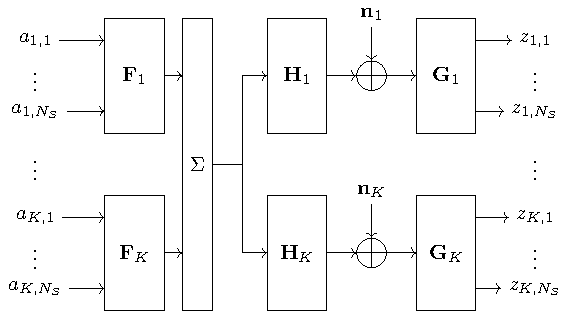
\includegraphics[width=\textwidth]{figures/background_material/04_mu_mimo_precoding/out/channel_original.pdf}
        \caption{}
        \label{fig:mu_mimo_original_channel}
    \end{subfigure}
    \hfill
    \begin{subfigure}{0.45\textwidth}
        \centering
        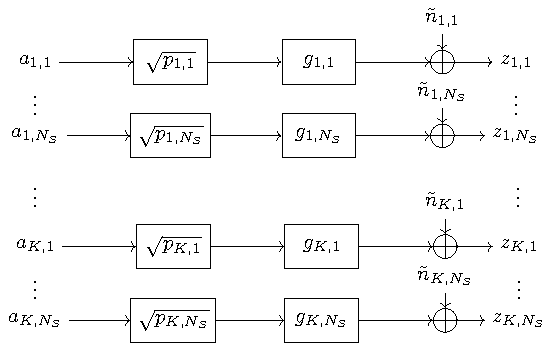
\includegraphics[width=\textwidth]{figures/background_material/04_mu_mimo_precoding/out/channel_decomposition.pdf}
        \caption{}
        \label{fig:mu_mimo_decoupled_channel}
    \end{subfigure}
    \caption[Channel decomposition of a \acs*{MU}-\acs*{MIMO} system]{A block diagram of the original \acs*{MU}-\acs*{MIMO} channel (a) and its decomposition into parallel Gaussian \acs*{SISO} subchannels (b), as achieved by the \acs*{ZF}--type precoding techniques.}
    \label{fig:mu_mimo_channel_decomposition}
\end{figure}

Figure~\ref{fig:mu_mimo_eff_subchannel_gain_distributions_8x2x4} reports the marginal \acp{pdf} for a single user in a system with $8$ transmit antennas at the \ac{BS} and $4$ two-antenna \acp{UT}, obtained through Monte Carlo simulations.
Because users with the same number of receive antennas are statistically symmetric, this user is representative for the full set of users.
For pure \ac{ZF}, the effective subchannel gains are given by $g_n=\big((\mathbf{H}\mathbf{H}^{\mathsf{H}})^{-1}\big)_{n,n}^{-1}$ and, under an \ac{i.i.d.} Rayleigh fading model, their distribution follows from the inverse-Wishart model~\cite{wishart_matrices_1, wishart_matrices_0}.
In particular, each $g_n$ is Gamma-distributed with shape parameter $\alpha = N_T-KN_R+1$ and rate parameter $\beta=1$.
For \ac{ZF} with a heuristic \ac{LSV} combiner and for \ac{BD} precoding, no analytical distribution is derived.

\begin{figure}[htb!]
    \centering
    \makebox[\textwidth][c]{%
        \begin{subfigure}{0.4\textwidth}
            \centering
            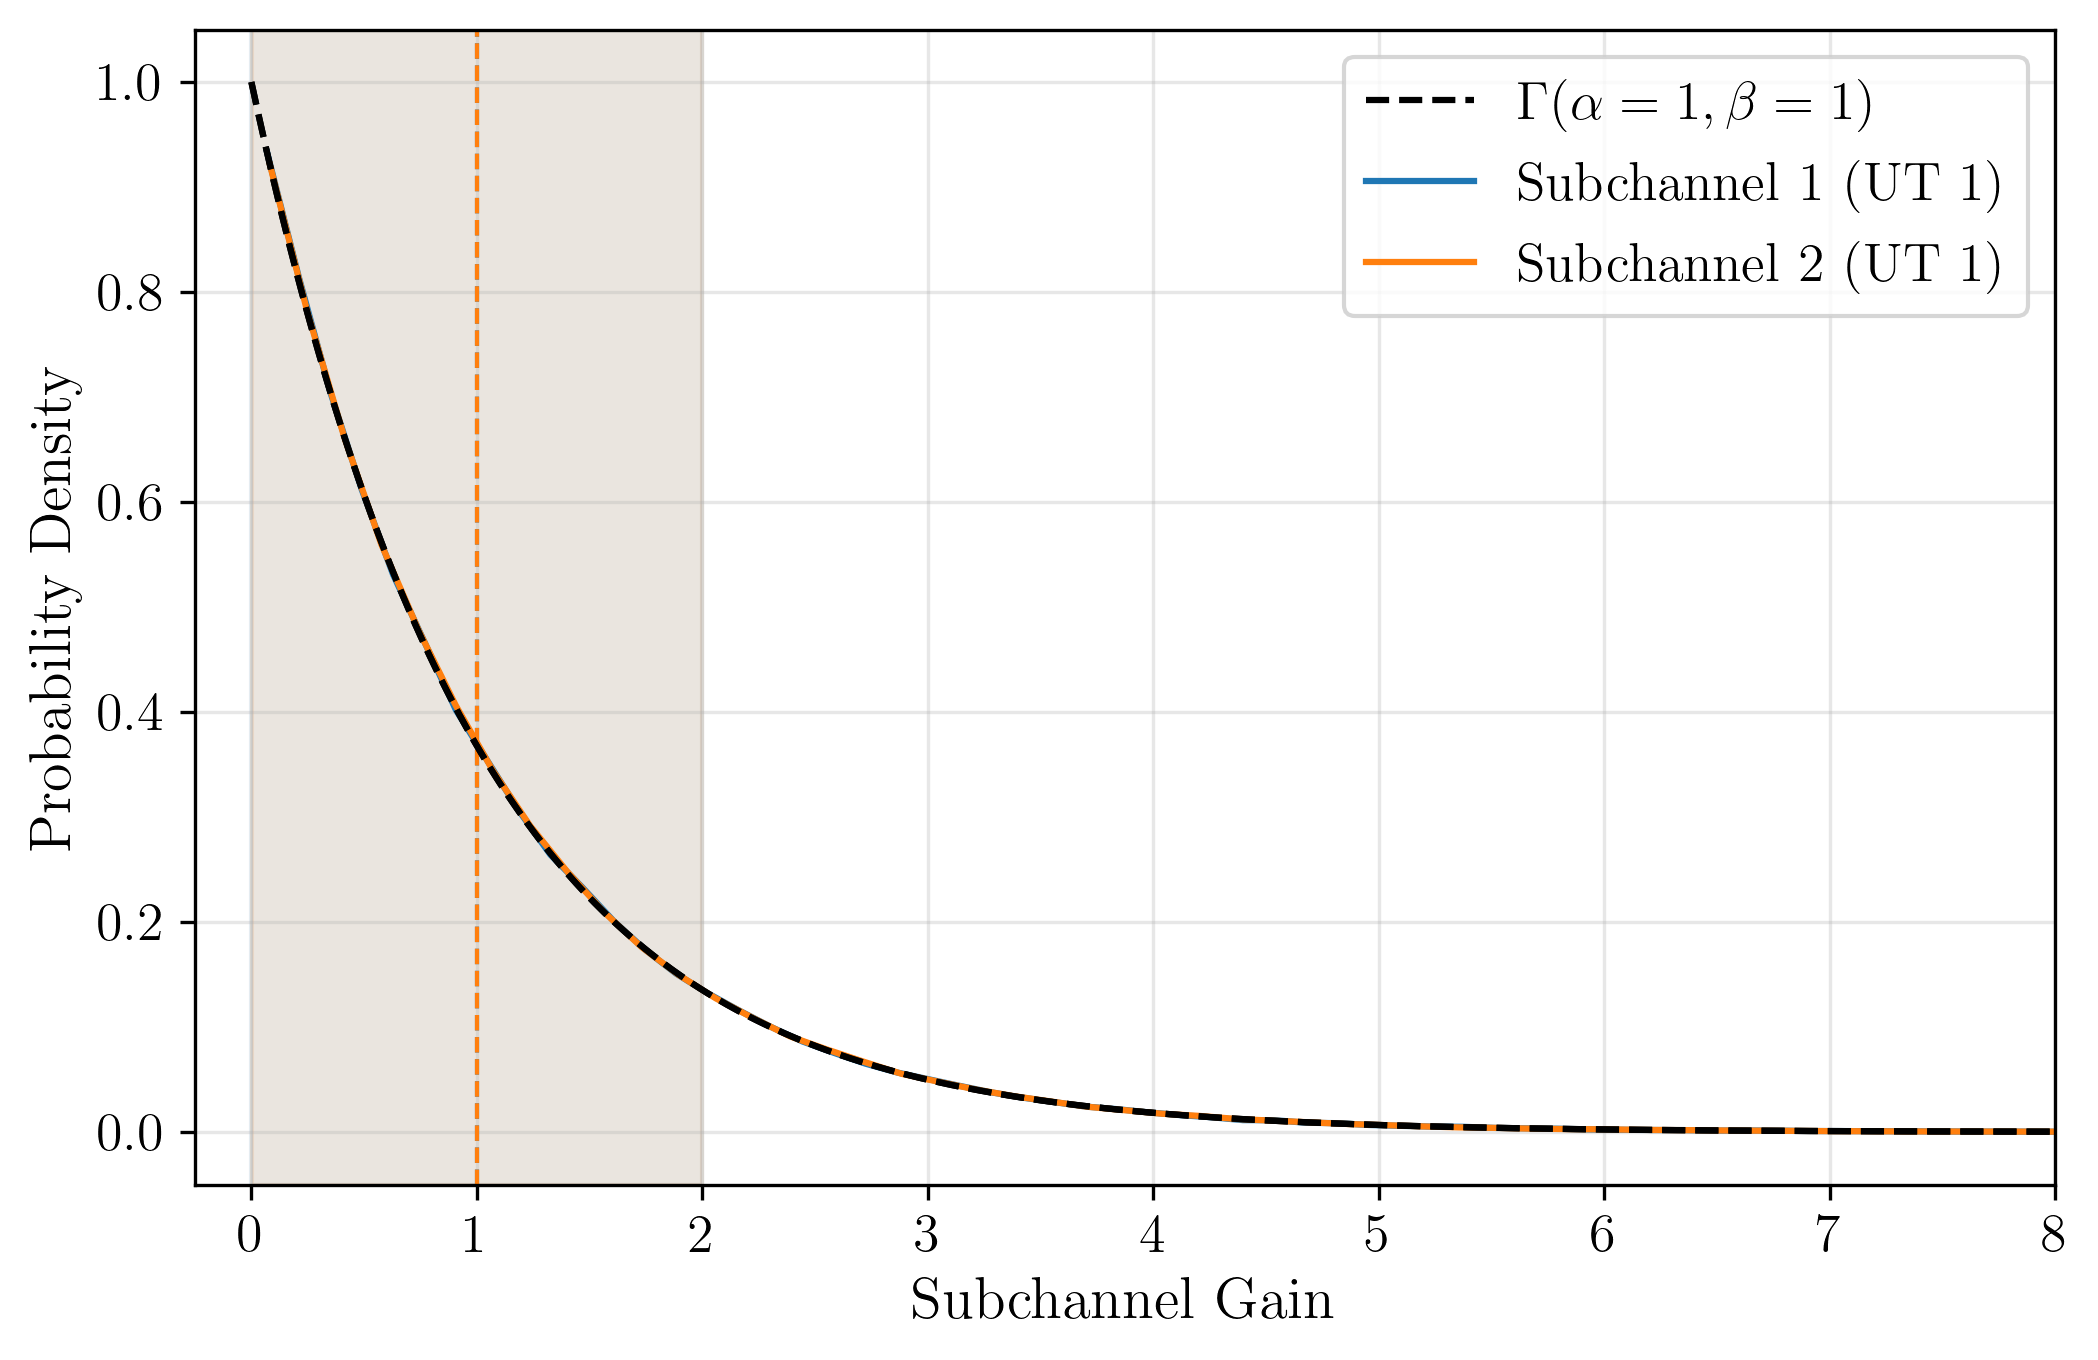
\includegraphics[width=\textwidth]{figures/background_material/04_mu_mimo_precoding/eff_subchannel_gain_distributions/ZF_8x2x4.png}
            \caption{\acs{ZF}}
            \label{fig:mu_mimo_eff_subchannel_gain_distributions_zf_8x2x4}
        \end{subfigure}
        \hfill
        \begin{subfigure}{0.4\textwidth}
            \centering
            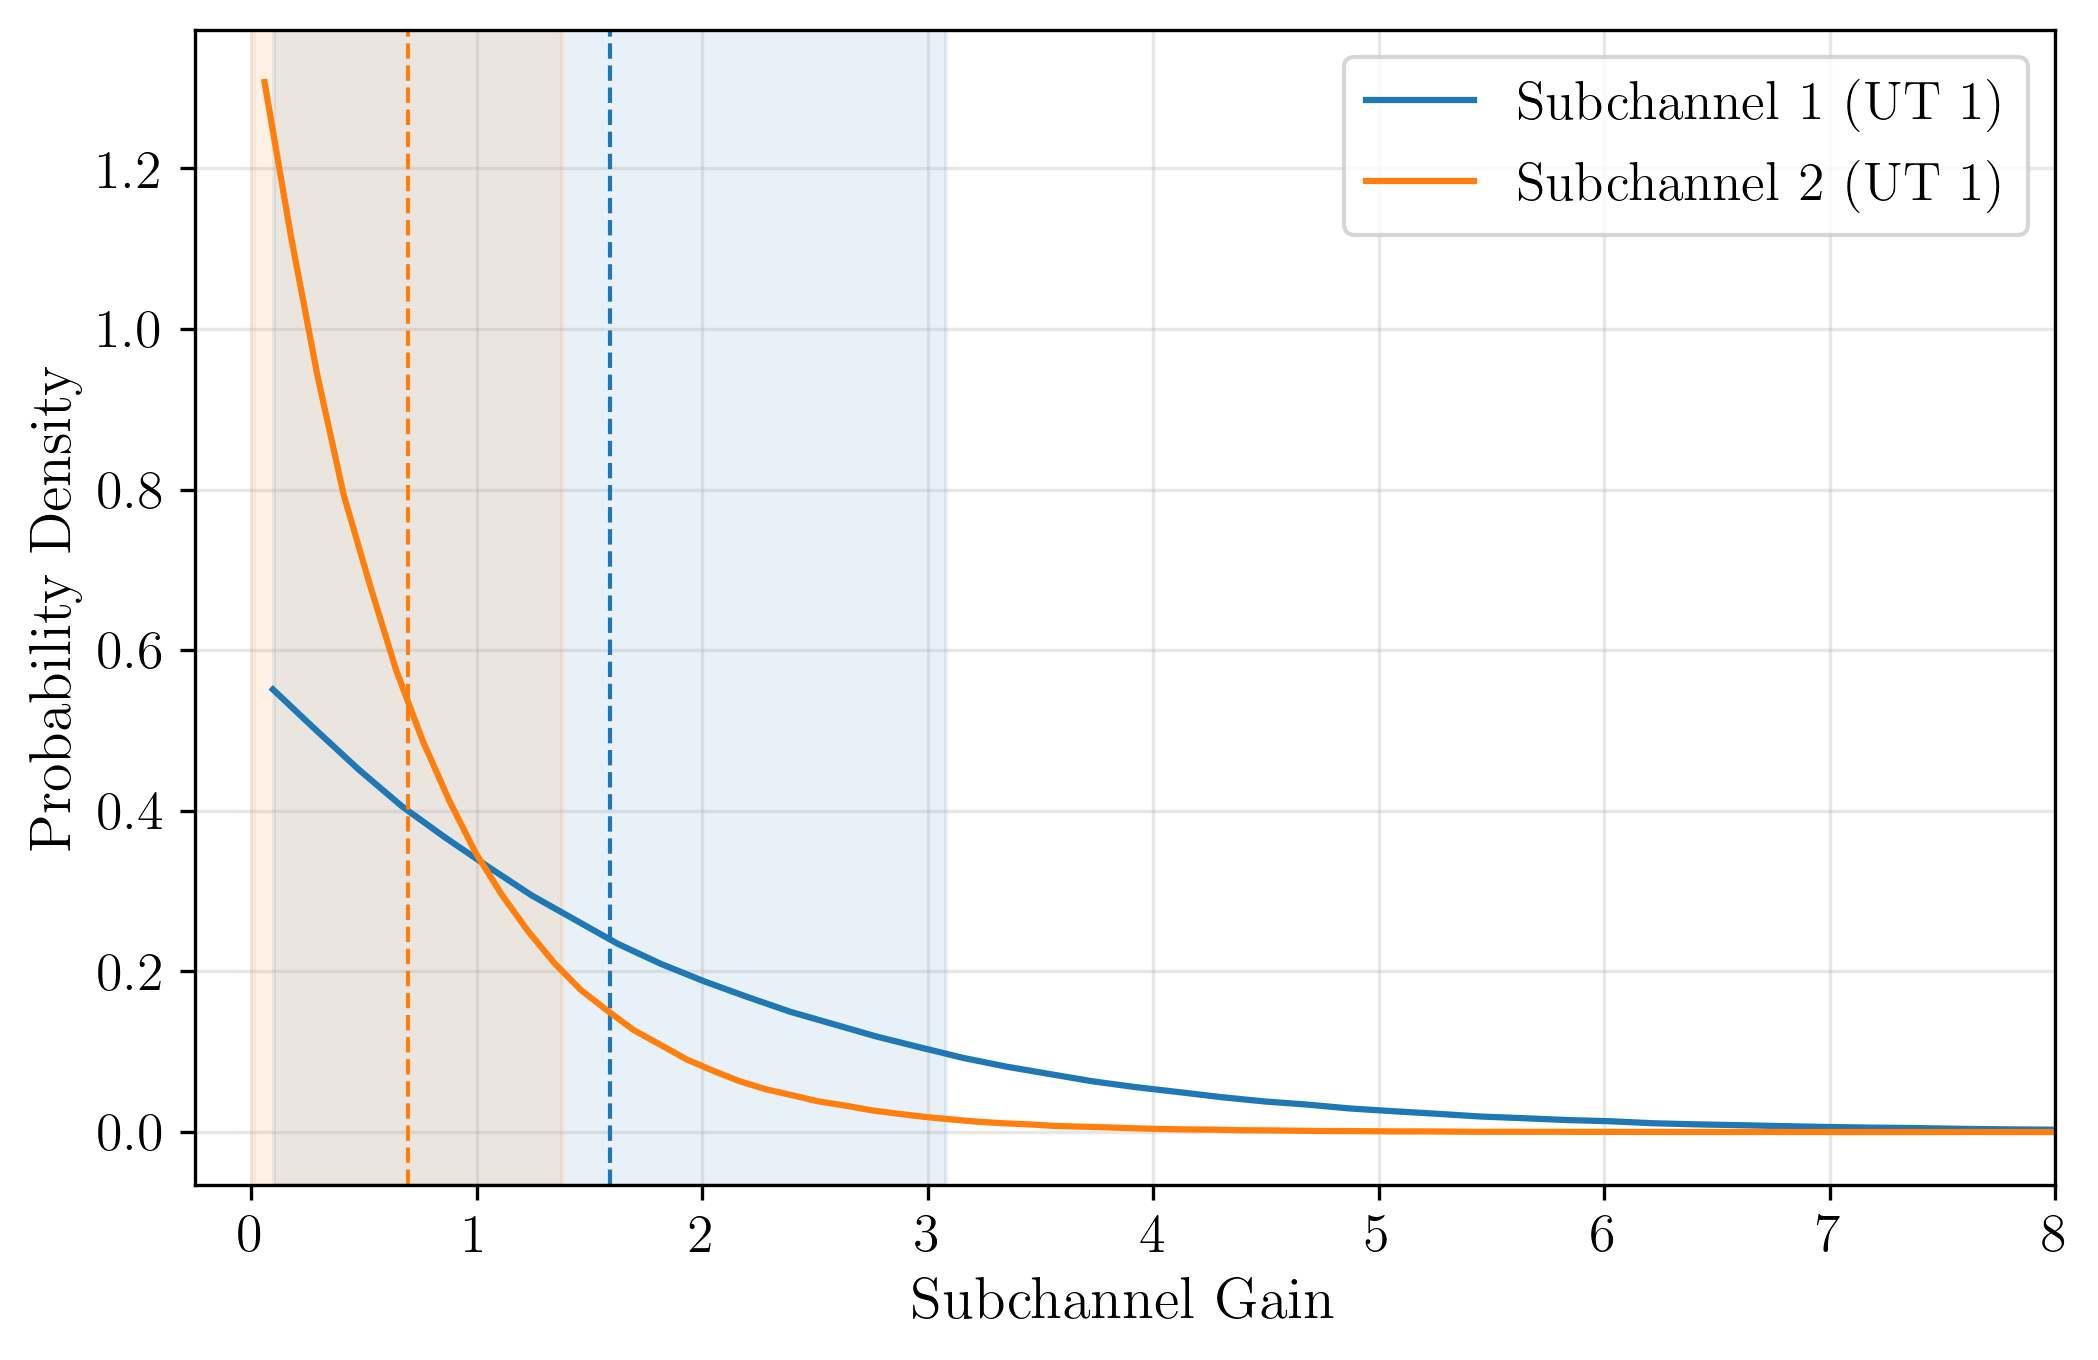
\includegraphics[width=\textwidth]{figures/background_material/04_mu_mimo_precoding/eff_subchannel_gain_distributions/ZFplusLSV_8x2x4.png}
            \caption{\acs{ZF} + \acs{LSV} Combiner}
            \label{fig:mu_mimo_eff_subchannel_gain_distributions_zf_lsv_8x2x4}
        \end{subfigure}
        \hfill
        \begin{subfigure}{0.4\textwidth}
            \centering
            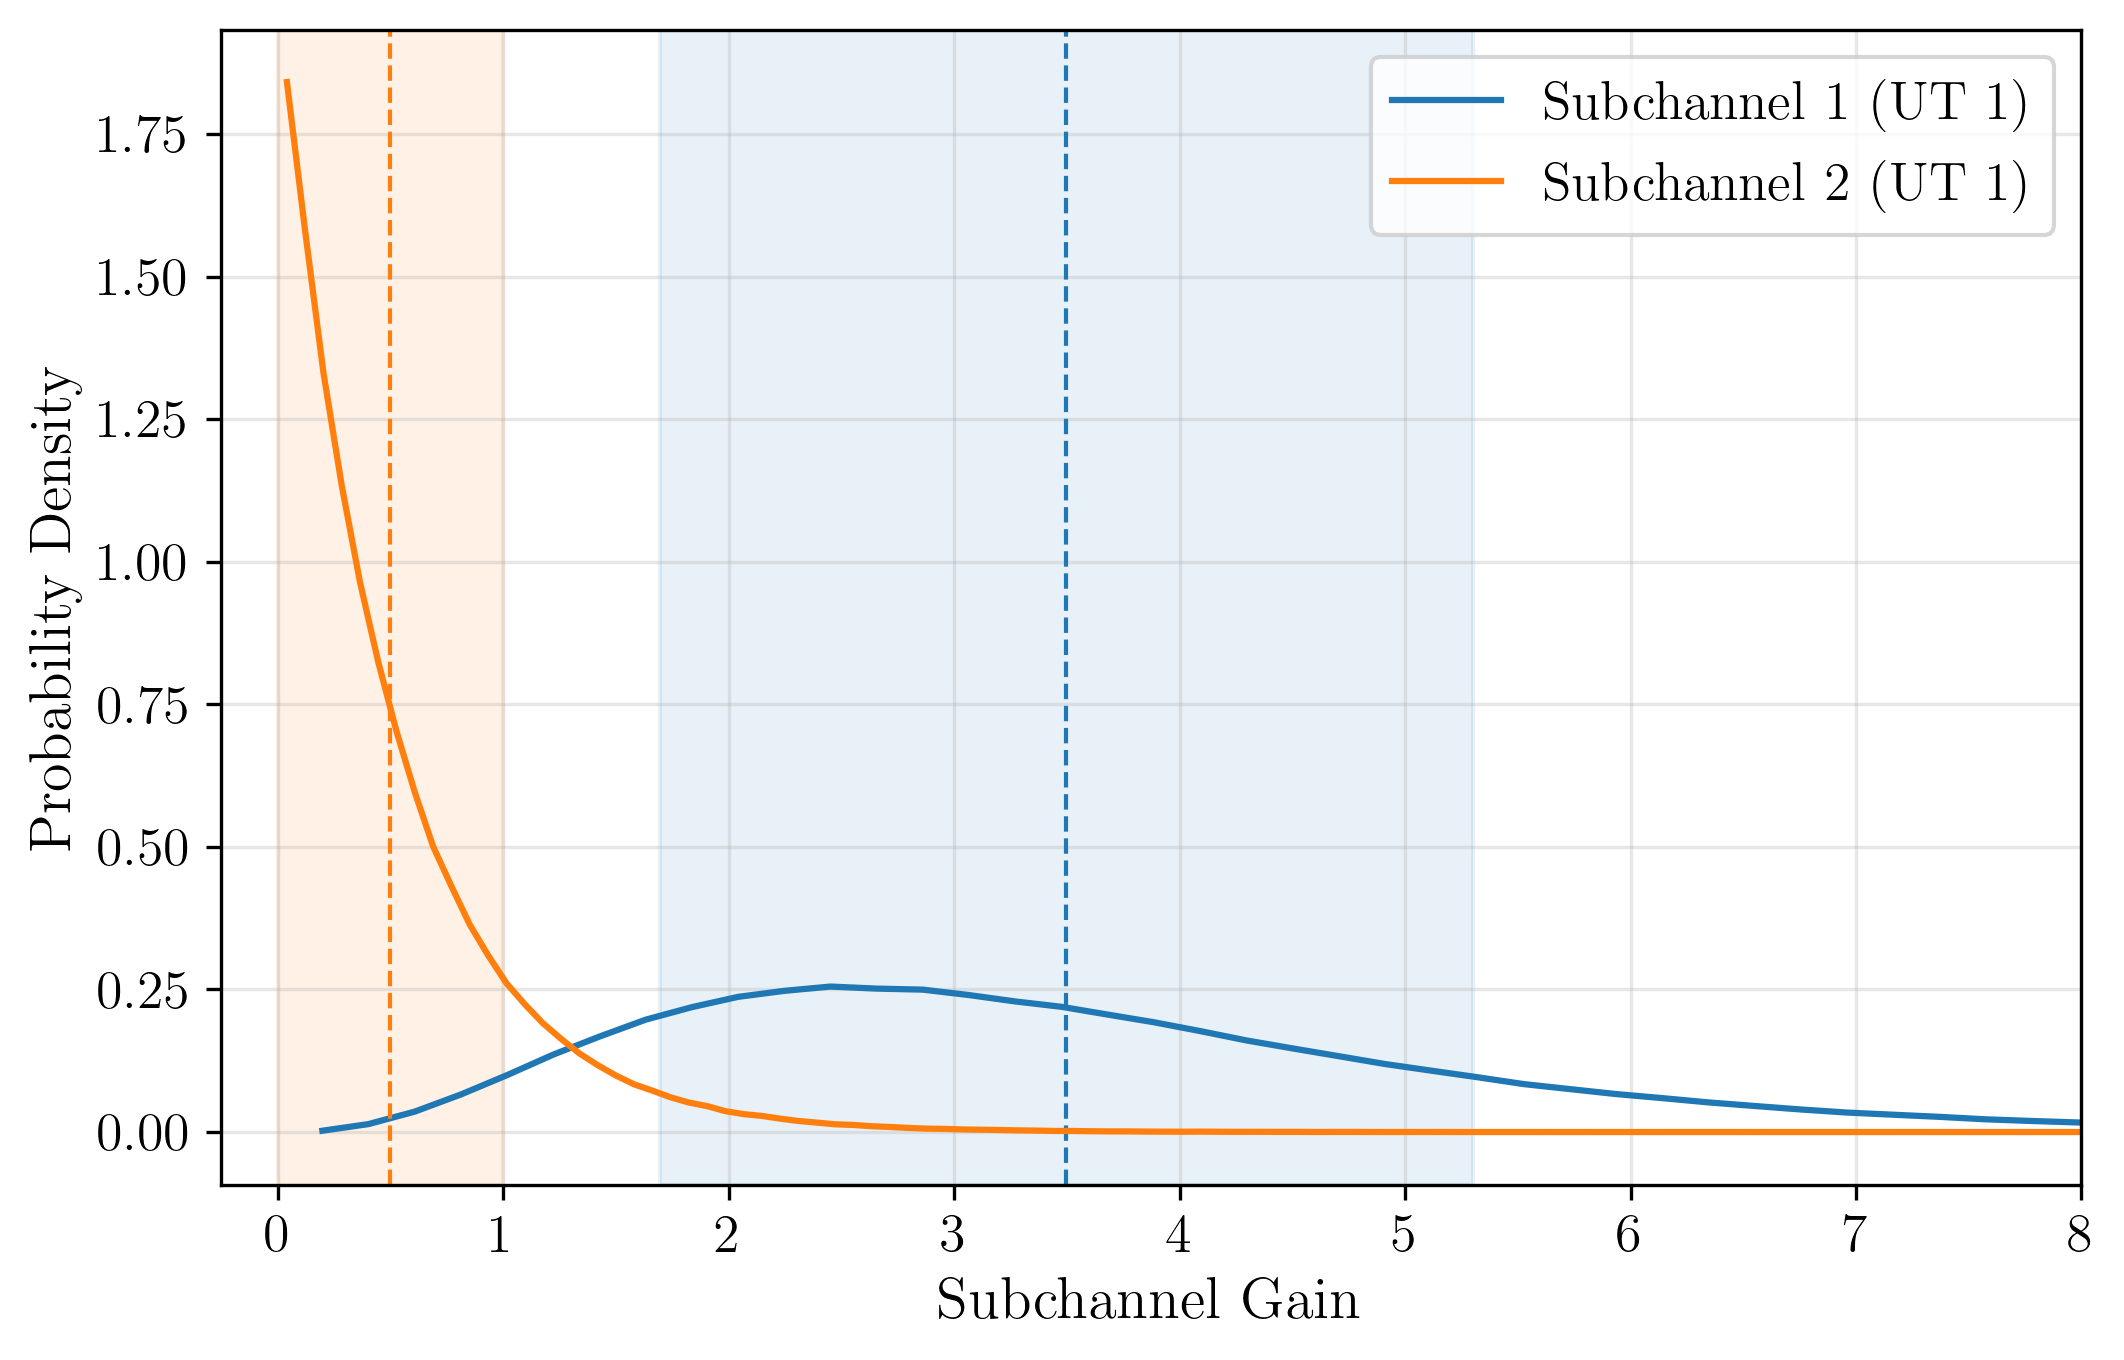
\includegraphics[width=\textwidth]{figures/background_material/04_mu_mimo_precoding/eff_subchannel_gain_distributions/BD_8x2x4.png}
            \caption{\acs{BD}}
            \label{fig:mu_mimo_eff_subchannel_gain_distributions_bd_8x2x4}
        \end{subfigure}
    }
    \caption[\acs{pdf} of the effective subchannel gains in a $8 \times \{2, 2, 2, 2\} \;$ \ac{MU}-\ac{MIMO} system]{The marginal \acsp{pdf} of the effective subchannel gains for a single \ac{UT} in a $8 \times \{2, 2, 2, 2\} \;$ \ac{MU}-\ac{MIMO} system, compared between the different \acs{ZF}--type precoding techniques.
    The expected value is indicated by a vertical dashed line, and the shaded area around the expected value corresponds to the standard deviation.}
    \label{fig:mu_mimo_eff_subchannel_gain_distributions_8x2x4}
\end{figure}
\begin{comment}
\begin{figure}[htb!]
    \centering
    \makebox[\textwidth][c]{%
        \begin{subfigure}{0.4\textwidth}
            \centering
            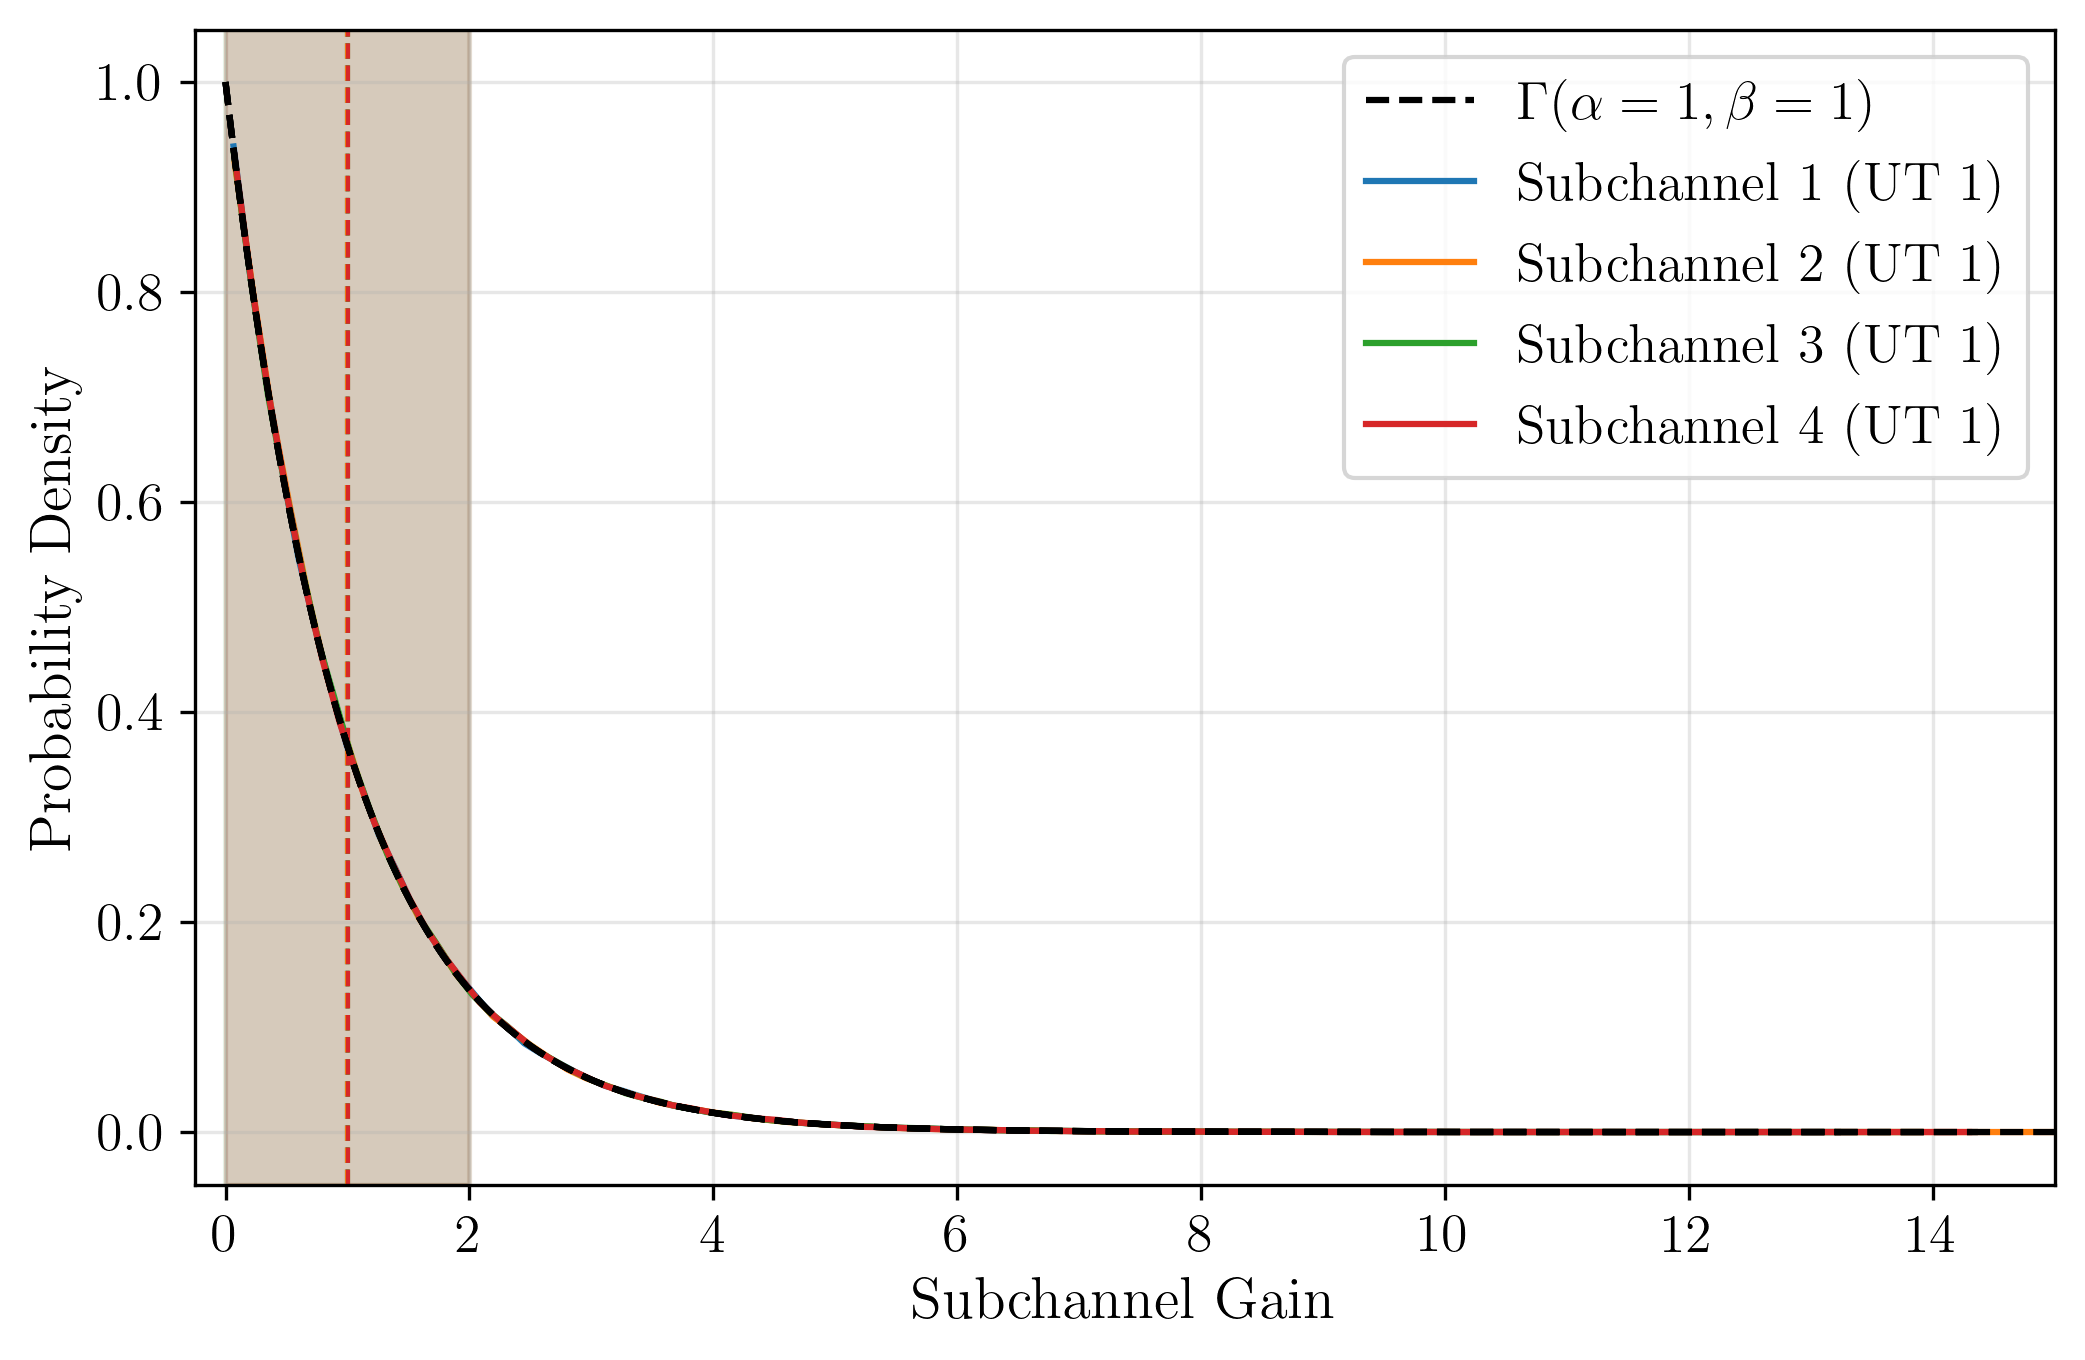
\includegraphics[width=\textwidth]{figures/background_material/04_mu_mimo_precoding/eff_subchannel_gain_distributions/ZF_8x4x2.png}
            \caption{\acs{ZF}}
            \label{fig:mu_mimo_eff_subchannel_gain_distributions_zf_8x4x2}
        \end{subfigure}
        \hfill
        \begin{subfigure}{0.4\textwidth}
            \centering
            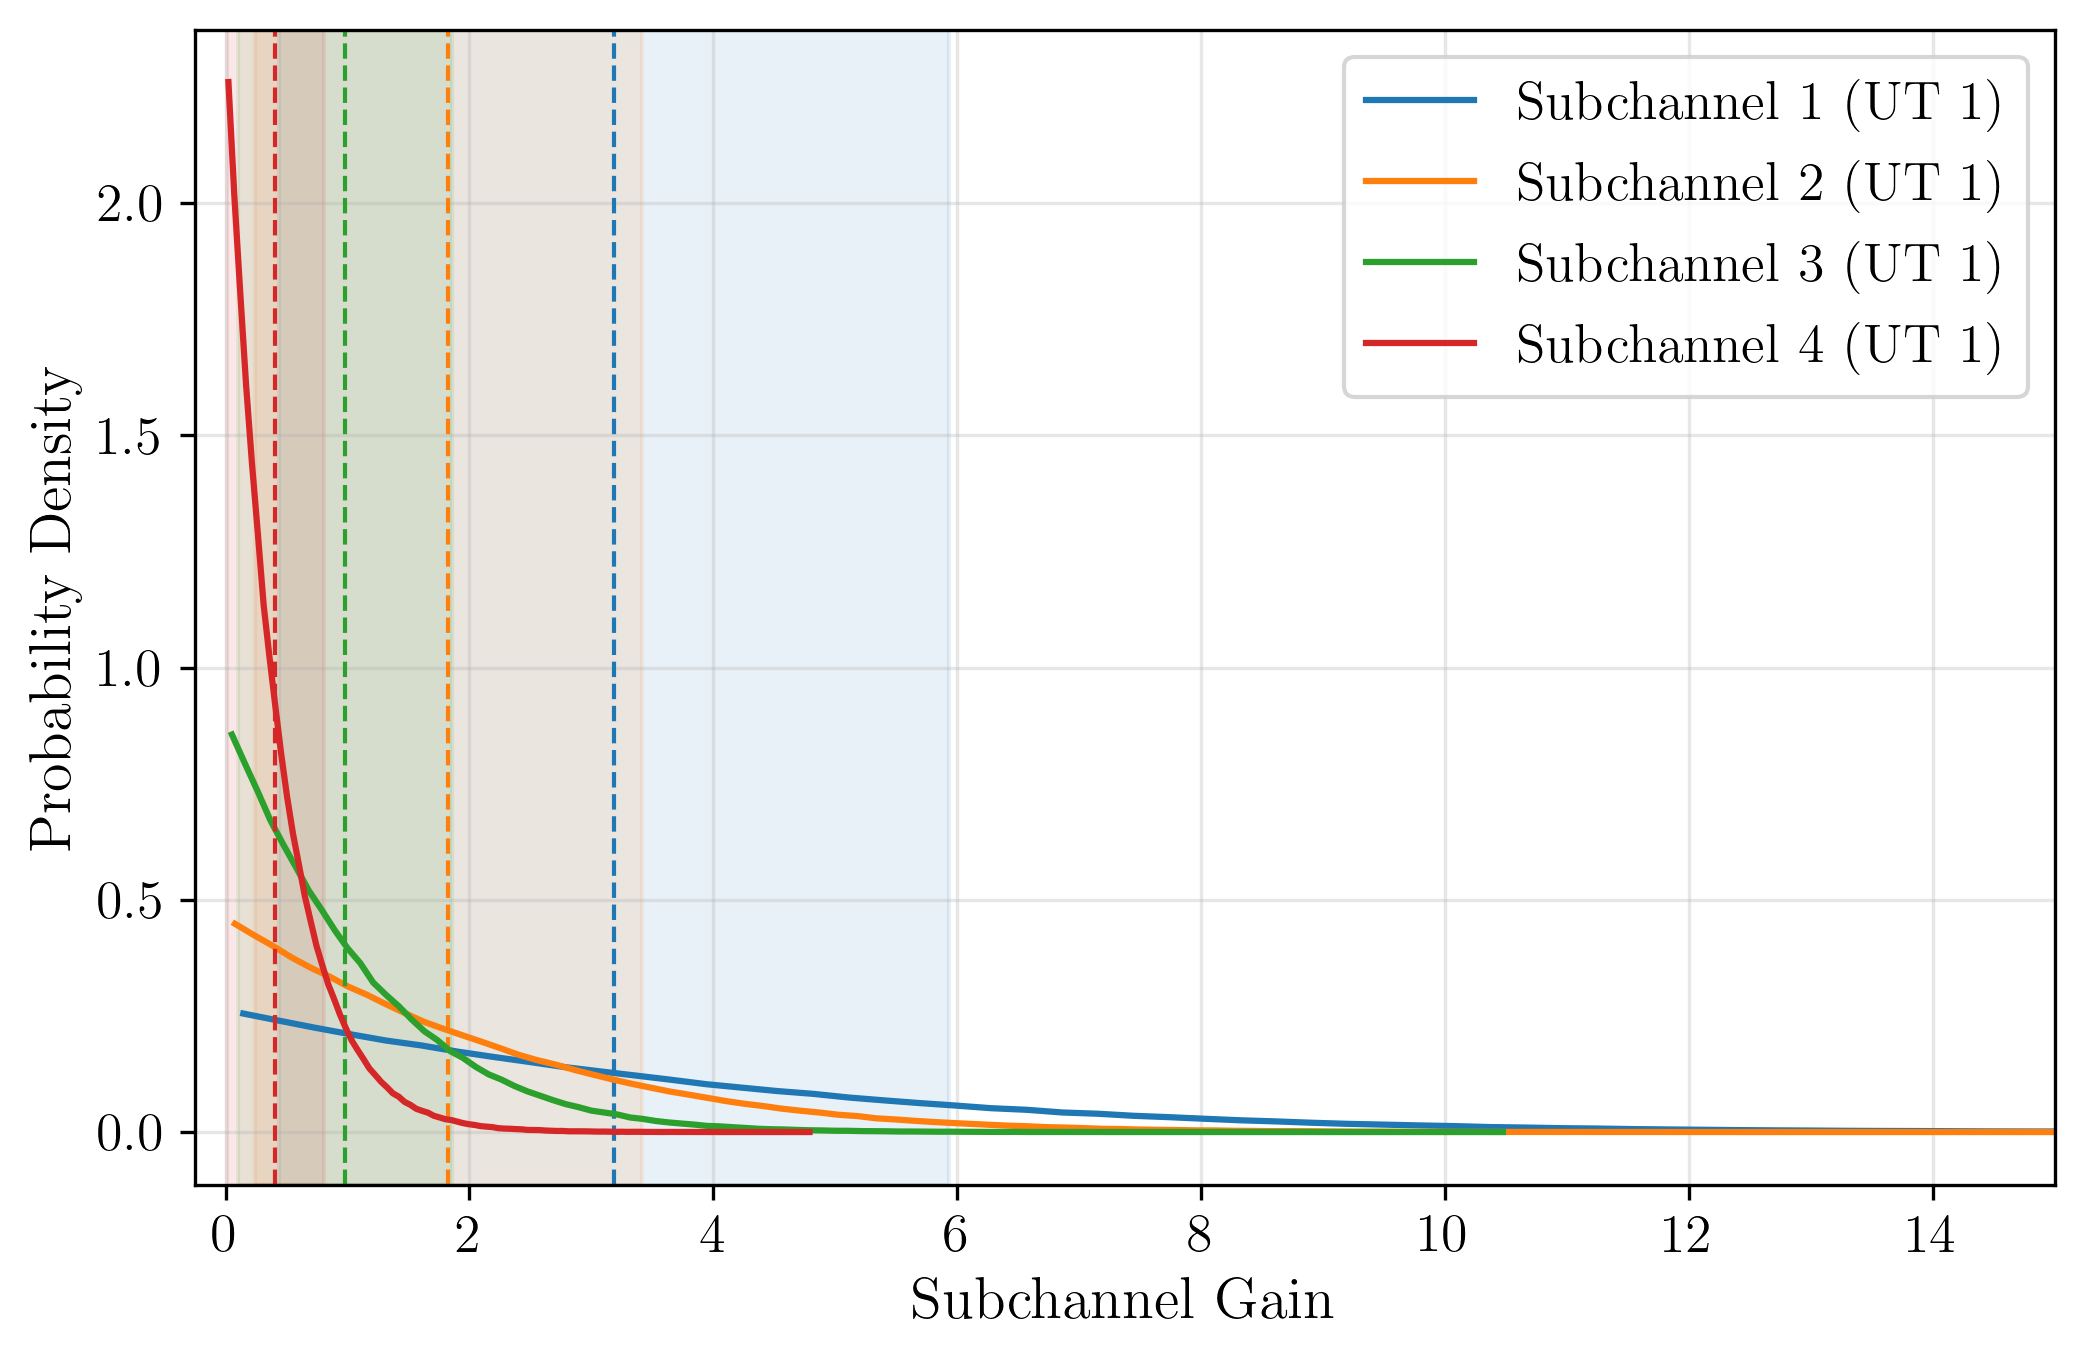
\includegraphics[width=\textwidth]{figures/background_material/04_mu_mimo_precoding/eff_subchannel_gain_distributions/ZFplusLSV_8x4x2.png}
            \caption{\acs{ZF} + \acs{LSV} Combiner}
            \label{fig:mu_mimo_eff_subchannel_gain_distributions_zf_lsv_8x4x2}
        \end{subfigure}
        \hfill
        \begin{subfigure}{0.4\textwidth}
            \centering
            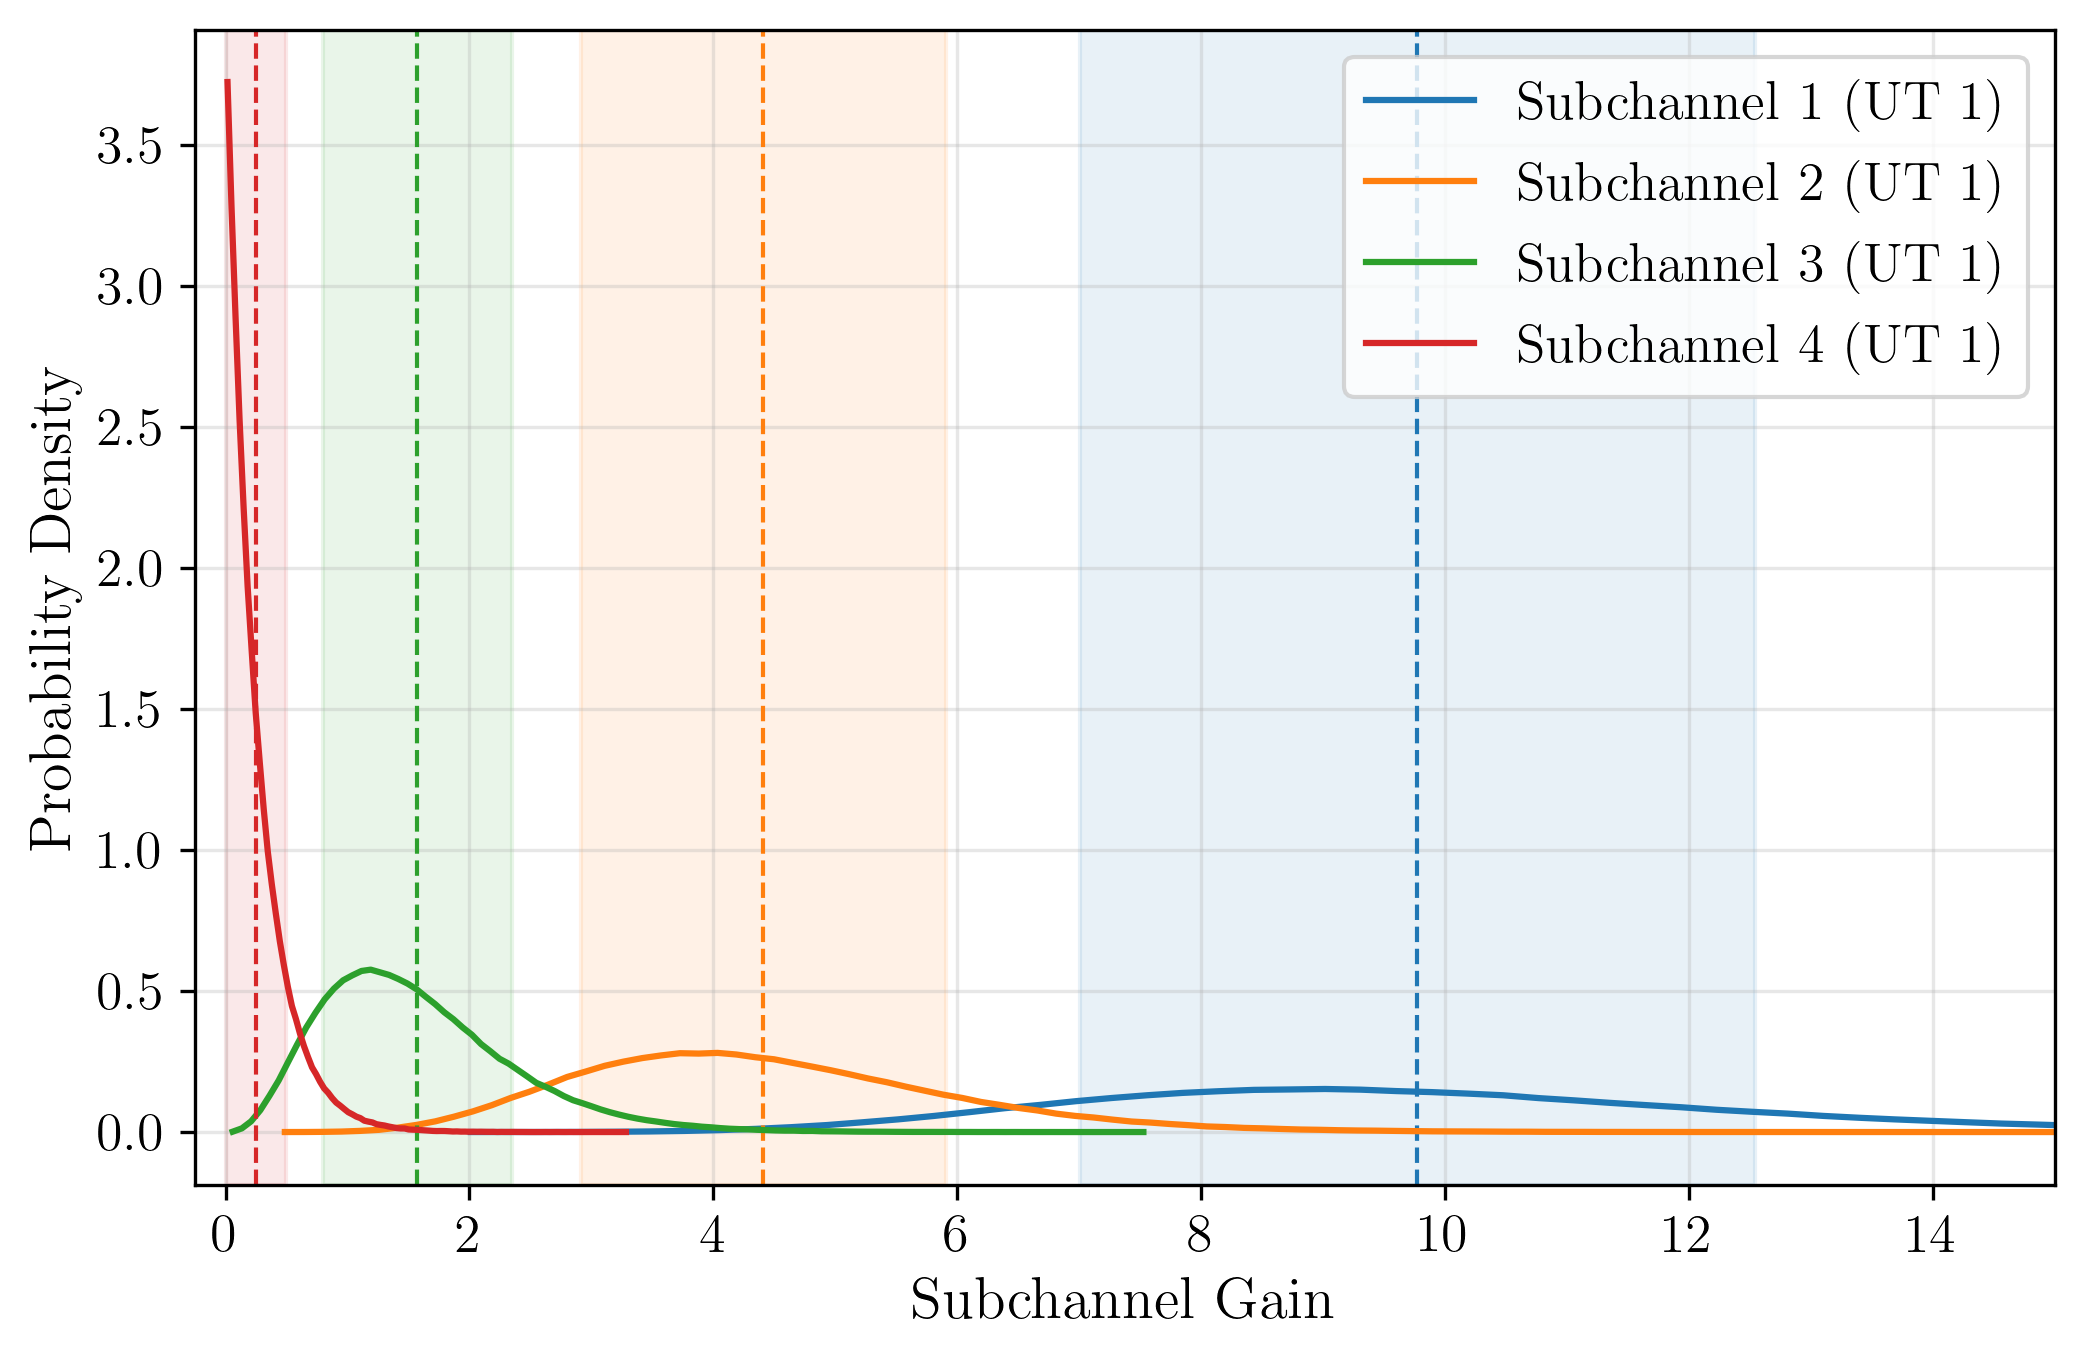
\includegraphics[width=\textwidth]{figures/background_material/04_mu_mimo_precoding/eff_subchannel_gain_distributions/BD_8x4x2.png}
            \caption{\acs{BD}}
            \label{fig:mu_mimo_eff_subchannel_gain_distributions_bd_8x4x2}
        \end{subfigure}
    }
    \caption[\acs{pdf} of the effective subchannel gains in a $8 \times \{4, 4\} \;$ \ac{MU}-\ac{MIMO} system]{Similar figure as Figure~\ref{fig:mu_mimo_eff_subchannel_gain_distributions_8x2x4}, now for a $8 \times \{4, 4\} \;$ \ac{MU}-\ac{MIMO} system}
\end{figure}
\end{comment}

For pure \ac{ZF} (Fig.~\ref{fig:mu_mimo_eff_subchannel_gain_distributions_zf_8x2x4}), the two subchannels of a single \ac{UT} have identical marginal distributions, consistent with the analytical result.
Adding the heuristic \ac{LSV} combiner (Fig.~\ref{fig:mu_mimo_eff_subchannel_gain_distributions_zf_lsv_8x2x4}) breaks this symmetry between the two subchannels.
The first combiner vector is aligned with the dominant left singular vector of $\mathbf{H}_k$, which concentrates the available receive-side spatial gain onto the dominant subchannel at the expense of the weaker one. This creates a slightly more favorable result compared to pure \ac{ZF}.
\ac{BD} precoding (Fig.~\ref{fig:mu_mimo_eff_subchannel_gain_distributions_bd_8x2x4}) achieves substantially larger gains for the dominant subchannel than those observed under the \ac{ZF} with \ac{LSV} combiner technique.
The sum of the expected subchannel gains is clearly the largest, due to the better utilization of the spatial degrees of freedom and the coordinated design.
Similar observations hold for other antenna configurations.

These differences in subchannel gain statistics translate directly into differences in achievable sum rate, as will be shown in the next section.

\subsection{Achievable Sum Rate Comparison}
\label{section:mu_mimo_sum_rate_comparison}
% ====================================
%   Achievable Sum Rate Comparison
% ====================================

Figure~\ref{fig:mu_mimo_sum_rate_comparison} compares the achievable \ac{SR} of all four precoding techniques for two fully loaded \ac{MU}-\ac{MIMO} configurations, where ``fully loaded'' means that the total number of receive antennas equals the number of transmit antennas ($K N_R = N_T$).
The two configurations differ only in how the receive antennas are distributed across \acp{UT}: four \acp{UT} with two receive antennas each in Fig.~\ref{fig:mu_mimo_sum_rate_comparison_8x2x4} and two \acp{UT} with four receive antennas each in Fig.~\ref{fig:mu_mimo_sum_rate_comparison_8x4x2}.

\begin{figure}[!hbt]
    \centering
    \begin{subfigure}{0.495\textwidth}
        \centering
        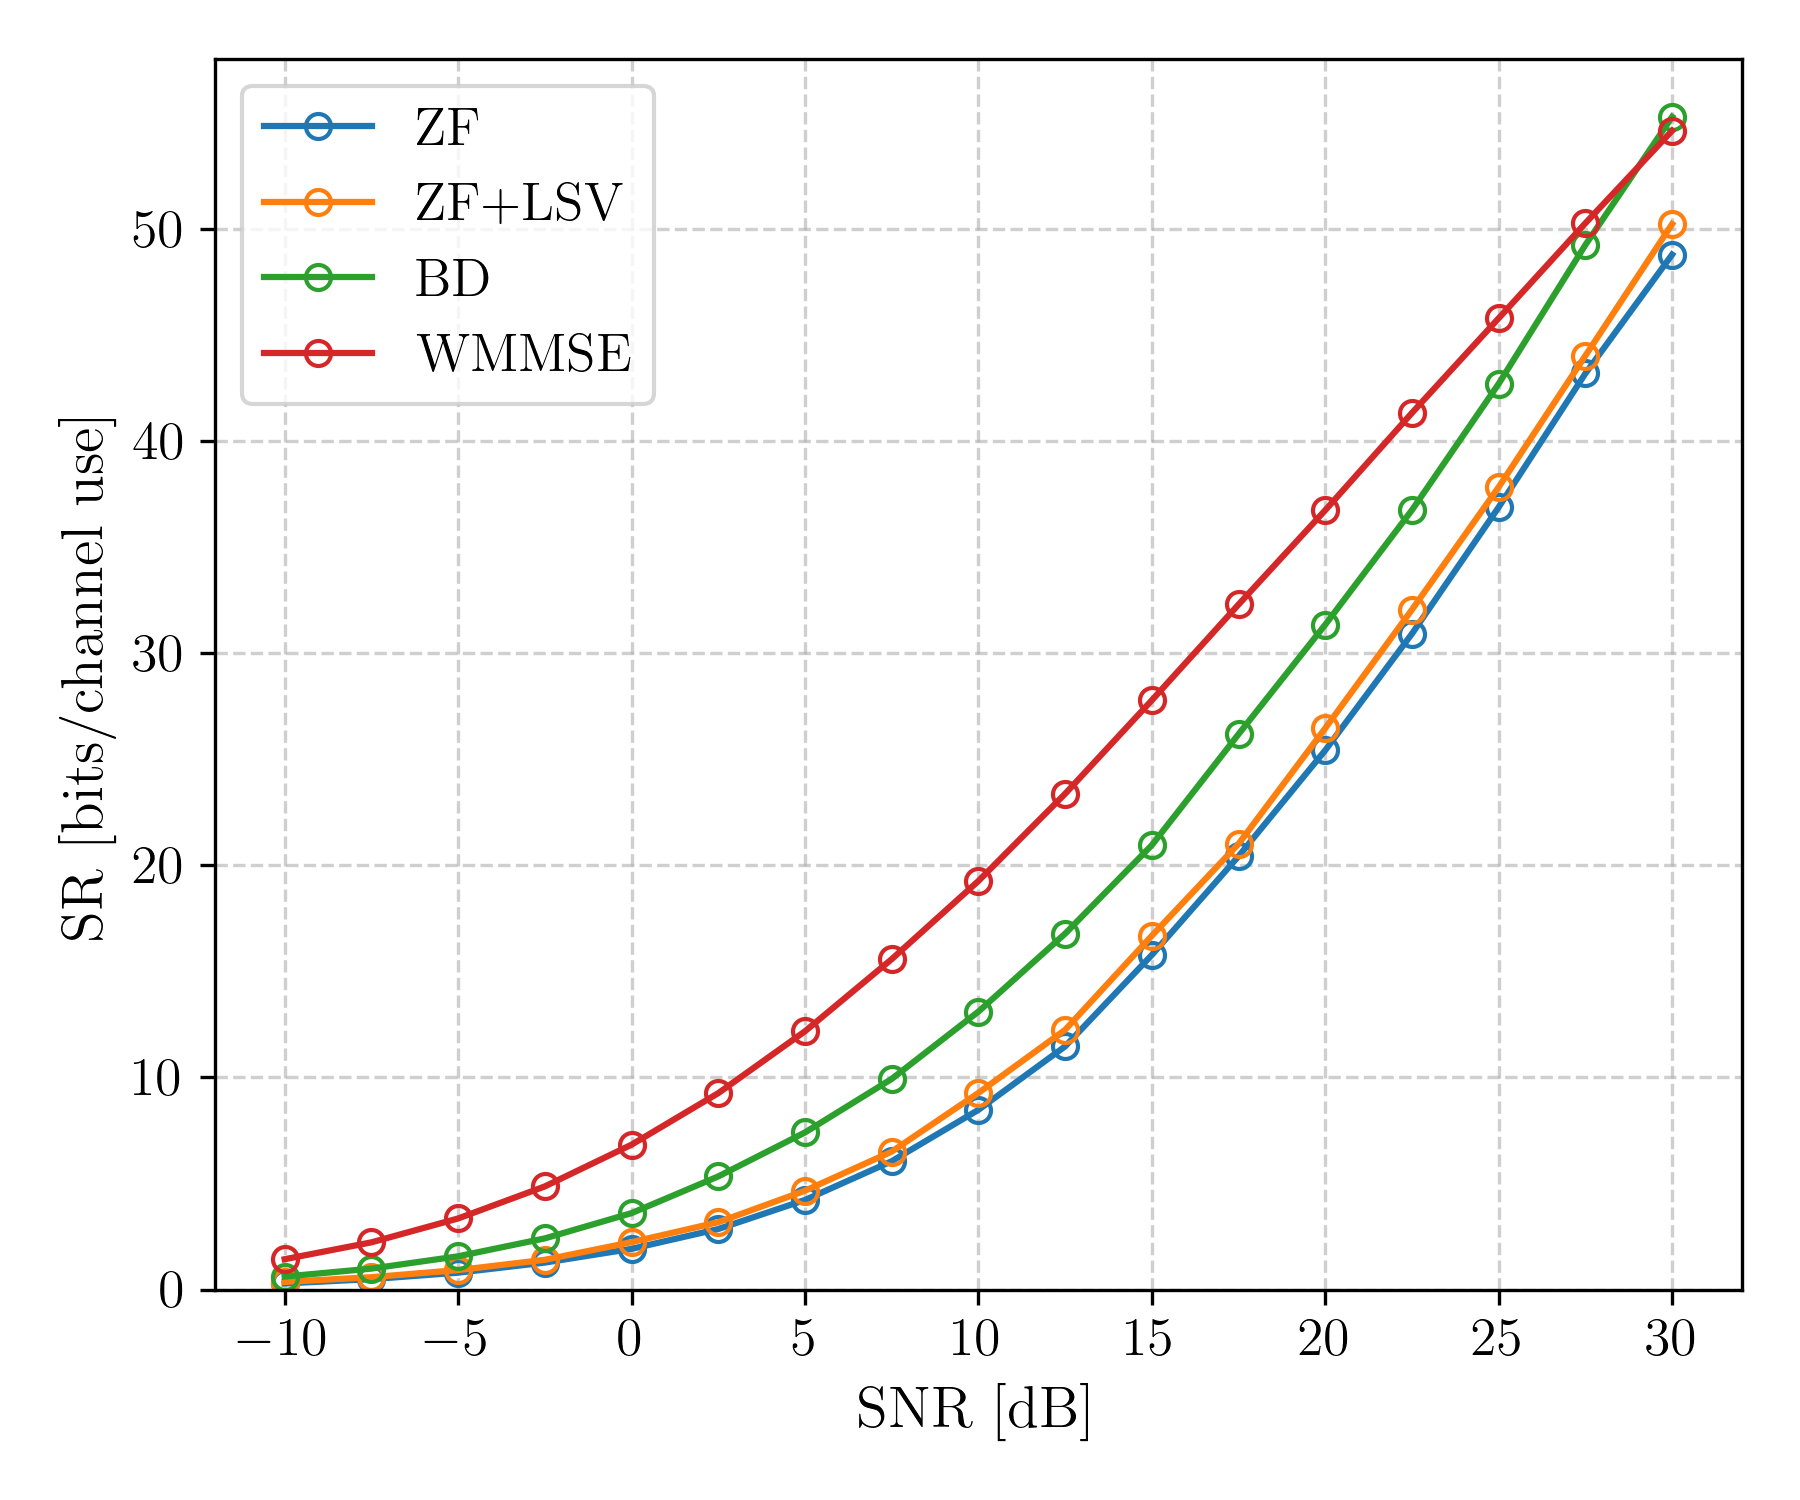
\includegraphics[width=\textwidth]{figures/background_material/04_mu_mimo_precoding/simulation_results/sr_comparison_8x2x4.png}
        \caption{$8 \times \{2, 2, 2, 2\}$ \ac{MU}-\ac{MIMO}}
        \label{fig:mu_mimo_sum_rate_comparison_8x2x4}
    \end{subfigure}
    \hfill
    \begin{subfigure}{0.495\textwidth}
        \centering
        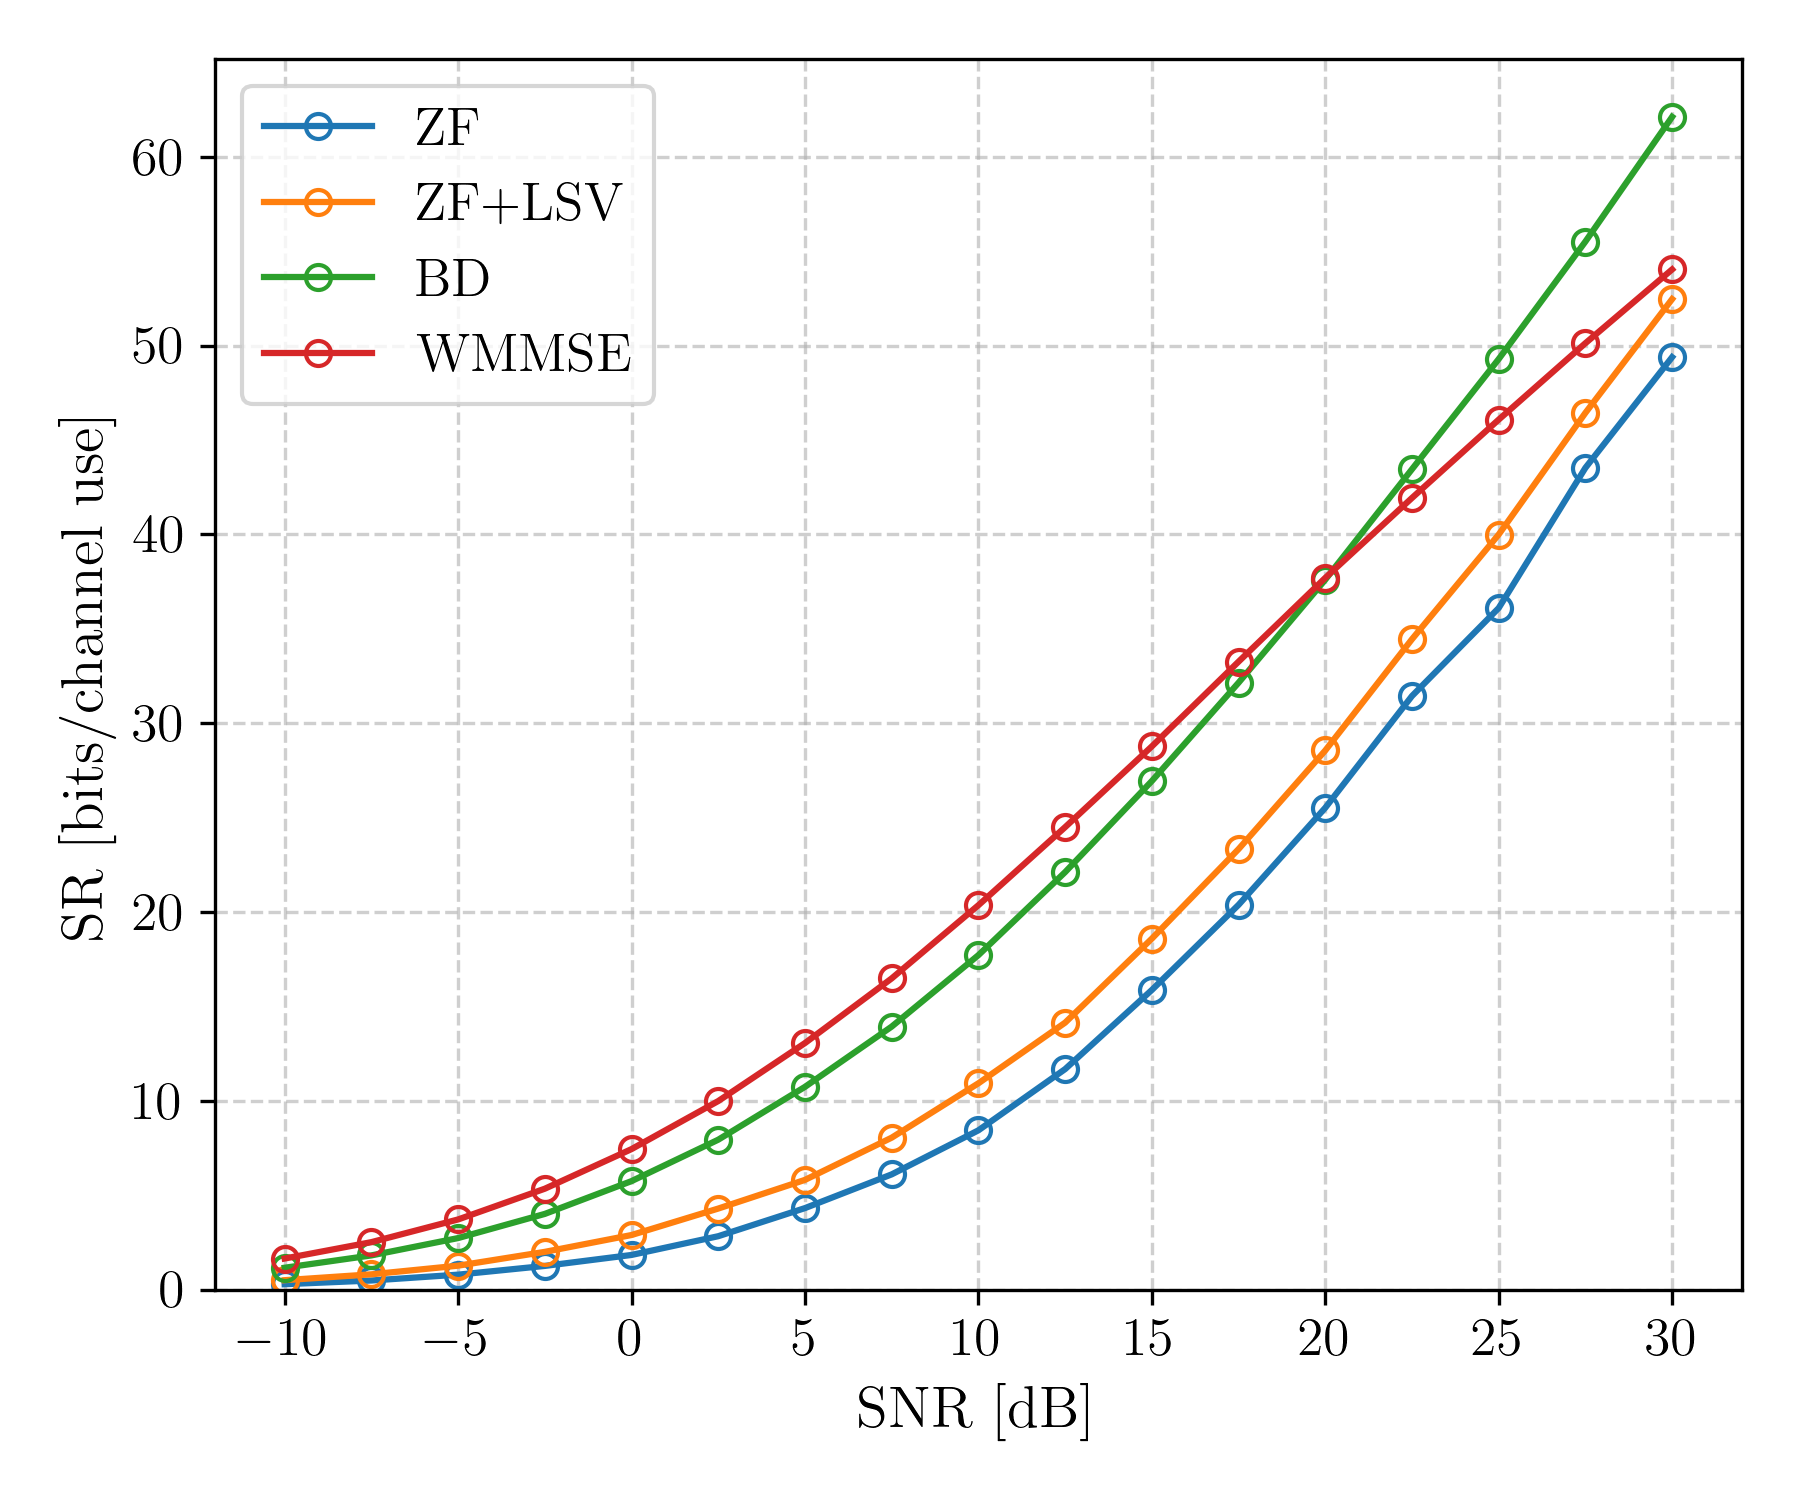
\includegraphics[width=\textwidth]{figures/background_material/04_mu_mimo_precoding/simulation_results/sr_comparison_8x4x2.png}
        \caption{$8 \times \{4, 4\}$ \ac{MU}-\ac{MIMO}}
        \label{fig:mu_mimo_sum_rate_comparison_8x4x2}
    \end{subfigure}
    \caption[Achievable \acs{SR} comparison of the different precoders in two \acs{MU}-\acs{MIMO} systems]
    {Comparison of the achievable sum rate for the considered \acs{MU} linear precoding techniques in two fully loaded \acs{MU}-\acs{MIMO} systems.
    The results are averaged over at least $1000$ \acs{i.i.d.} Rayleigh channel realizations.}
    \label{fig:mu_mimo_sum_rate_comparison}
\end{figure}

In both configurations, the ranking
$$
SR_{\text{WMMSE}} > SR_{\text{BD}} > SR_{\text{ZF}+\text{LSV}} > SR_{\text{ZF}} 
$$
holds at moderate \ac{SNR}, consistent with the increasing level of design flexibility across the four methods.
Pure \ac{ZF} imposes the strictest constraints, requiring the precoder to invert the full compound channel matrix with no receiver-side processing.
\ac{ZF} with \ac{LSV} combining retains the same precoder structure but introduces receive-side spatial processing.
\ac{BD} further relaxes the structural constraints from per-stream to per-user orthogonality and exploits receiver combining through a coordinated design, yielding a substantial gain in achievable \ac{SR}.
\ac{WMMSE} places no structural constraint on the precoder and directly optimizes the \ac{WSR}, achieving the highest \ac{SR} at moderate \ac{SNR}.
The performance differences manifest as a horizontal \ac{SNR} offset rather than a change in growth rate, because all four techniques achieve the same multiplexing gain.

A notable exception to the above ranking occurs at very high \ac{SNR} in the $8 \times \{4,4\}$ configuration, where \ac{BD} eventually overtakes \ac{WMMSE}.
This crossover arises because \ac{BD} approaches the globally optimal solution for the maximum-information-rate criterion as \ac{SNR} grows~\cite{BD_precoding_0}, while \ac{WMMSE} may converge to a suboptimal local optimum in this regime.

Comparing the two configurations also reveals how the distribution of receive antennas affects performance.
For pure \ac{ZF}, the two curves are virtually identical: since no receiver combining is applied and the total number of receive antennas is the same, the achievable \ac{SR} depends only on the compound channel and is unaffected by how the antennas are grouped across \acp{UT}.
For \ac{ZF} with \ac{LSV} combining, \ac{BD} and \ac{WMMSE}, concentrating the receive antennas on fewer \acp{UT} yields a consistently higher \ac{SR}.
The benefit of concentrating antennas is more pronounced for \ac{BD} than for \ac{ZF}+\ac{LSV}, which reflects the fact that the coordinated \ac{BD} design makes fuller use of the per-user spatial degrees of freedom than the non-coordinated \ac{LSV} heuristic.

The simulation results confirm the position of \ac{WMMSE} as the state-of-the-art linear \ac{MU}-\ac{MIMO} precoding technique under the maximum-\ac{SR} criterion.
\ac{BD} provides a close-to-optimal coordinated alternative that does not require iterative optimization, while \ac{ZF}+\ac{LSV} offers a low-overhead non-coordinated baseline.
The choice between these techniques in practice therefore involves a trade-off between achievable \ac{SR}, computational complexity, and signaling overhead.
In the next chapters, performance evaluations are carried out using the \ac{WMMSE} precoder.
